\section{Numerical simulation algorithms} % TODO
\subsection{Finite-difference time-domain} % TODO
\paragraph{Algorithm desciption} %{{{
Finite-difference time-domain (FDTD) is one of the simplest methods for solving partial differential equations (PDE). The simulation volume is initialized as an array in the computer memory, each element of which corresponds to a \textit{voxel} in the orthogonal grid. When FDTD is applied to solve the Maxwell equations in three dimensions, six real numbers per voxel describe the electric and magnetic vector fields, another static scalar array describes the permittivity of the structure and additional arrays may correspond other physical quantities, such as material conductivity, material polarizabilities and polarizations etc. Two-dimensional computations can reduce the number of arrays thanks to symmetry.

The actual computation is realized in consecutive time steps as an explicit arithmetic operation on each voxel, taking into account only the field values in the neighboring voxels and in the previous time step. This corresponds to iterating equations (\ref{eq_me3}), (\ref{eq_me4}) and (\ref{eq_ce}). % unclear - specify the field update routine exactly
Most of the computation time is thus occupied by a simple and unconditional loop repeatedly updating all voxels, which allows to fully employ the processor cache and facilitates multi-processor parallelisation. FDTD is applicable to (possibly non-linear) problems where either the temporal evolution of the fields is searched for, or for linear systems where a frequency-domain response function can be found by Fourier-transforming the time-domain response. 
\begin{figure}[h] \caption{A warning} \label{fg_parental} \centering 
	
\includegraphics[width=5cm]{img/Parental_Advisory_label.pdf}
\end{figure}

The time-stepping routine has the same computing cost in empty vacuum as inside a complex structure. Grid-based methods such as FDTD are therefore most efficient to problems where a structure has relatively complex shape, but its smallest features are no more than two or three orders of magnitude smaller than the simulation size. In contrast, an accurate-enough simulation of a structure that has some few very fine features surrounded by big empty space would require excessively high resolution, often resulting in the great majority of the voxels being inefficiently used in space where the high resolution is not needed. Other methods, % TODO discussed below
such as Finite-element method or Boundary-element method, would be preferable for such cases.

As is widely used in the later chapters,  %% TODO illustrate it below!
simulations of a wave propagating in any periodic structure can make use of the periodic boundaries of the simulated volume, so that only one unit cell has to be computed to get result of an infinite structure. The unit cells of periodic structures discussed in this thesis have smallest features not less than two orders of magnitude smaller than the unit cell size, and besides one is often interested in obtaining the whole spectrum information, so FDTD was an optimal tool for this task.
%}}}
\paragraph{Spatial discretisation} %{{{
The discretisation of the grid and of the time stepping introduces an error that obviously manifests in imprecise description of the structure being simulated (\textit{staircasing}) and also in the \textit{numerical dispersion} \cite{taflove2005book}, that is, in deviation of the light speed from the correct one at higher frequencies.  % todo is something missing?
\begin{figure}[h] \caption{\textbf{a)}, \textbf{b)} Different two-dimensional grids are used for different polarizations of the fields. \textbf{c)} The three-dimensional Yee grid. The electric field components are expressed in the centers of the cube edges which they are parallel to, whereas the magnetic components are expressed in the centers of the cube which they are perpendicular to. Note the electric and magnetic fields are completely equal in this scheme; the description in terms of edges and faces could be interchanged if the brown cube was taken as the elementary one.} \label{fg_fdtd_yee} \centering 
	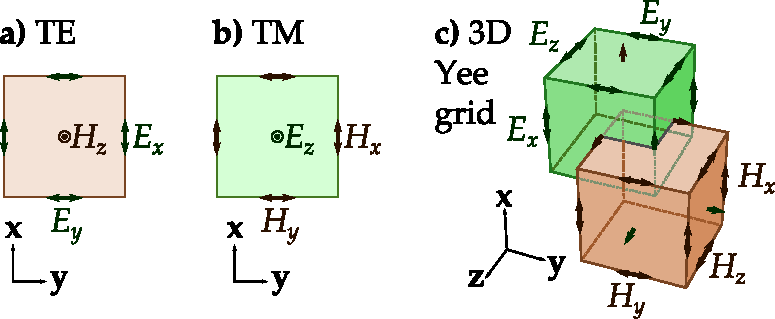
\includegraphics[width=10cm]{img/FDTD_Yee_grid_2d-3d.pdf}
\end{figure}

The error due to the numerical dispersion is in most FDTD implementations reduced from first to second order ($\propto \Delta x^{-2}$ with regards to the voxel size $\Delta x$) by using a \textit{staggered grid}, which in three dimensions is also known as Yee grid \cite{yee1966numerical}. All six field components are expressed in different points within the voxel, as is illustrated in Fig. \ref{fg_fdtd_yee}c with the upper left (green) cube denoting the elementary one. 
%This is similar to the advantage of trapezoid integration instead of direct summation. % TODO figure
Likewise, the update of electric and magnetic fields have to be interlaced also in time (as a so-called \textit{leapfrog} process). When accessing the field values at a given position and time, each field component has to be properly averaged between nearest points in the grid, and between nearest update times.


By adequate averaging of permittivity on the boundaries of materials, this error can likewise be reduced to the quadratic order with regards to $\Delta x$. Various averaging approaches have been studied in the literature \cite{oskooi2010meep}. Arithmetic averaging of permittivity with weight proportional to the voxel volume occupied by the material is perhaps the most intuitive one, but it often gives wrong results, and  sometimes it is even worse than no averaging at all \cite{farjadpour2006improving,deinega2007subpixel}. In case of a single planar interface of two different materials under general orientation, the arithmetic average of the permittivities $\varepsilon_r$ is correct only for electric field component \textit{parallel} with the interface, whereas the component \textit{perpendicular} to the interface requires instead to apply this weighted averaging to the reciprocal value of permittivity, $\varepsilon_r^{-1}$. Such an approach is extremely accurate for all interfaces with low curvature, but requires the FDTD simulation to define the permittivity as a $3\times 3$ tensor array (even in the simple case of isotropic materials being used). The situation gets even more  complicated if the materials have dispersive permittivity, where also the weighting coefficients of both media need to be frequency-dependent, and another sophisticated approach has to be employed \cite{deinega2007subpixel,hamm2013dispersive}. Such a level of elaboration easily leads to computation costs that may outweight the benefit of averaging, and accordingly no averaging was used for the simulations presented in this thesis. 

Generally, the effect of discretization in FDTD can be easily identified by comparing results from two simulations that only differ by the grid resolution. It is a good practice to verify that such an error is negligible whenever a new simulation is tested.
%}}}

\paragraph{Temporal discretisation} %{{{
While the spatial resolution $\Delta x$ can be relatively freely set depending on the accuracy expected by the user, the \textit{temporal resolution} $\Delta t$ is related to $\Delta x$ by rules that will be discussed below. Generally, if $\Delta t$ is set too high, the simulation will get numerically unstable, yielding unrealistic or even infinite values.  %  slowing down the computation and

In the literature, one often encounters that instead of description in terms of $\Delta t$, the \textit{Courant factor} $S$ is used:
\begin{equation} S~= \frac{c \Delta t}{\Delta x}, \label{eq_courant}\end{equation}
In words, the Courant factor $S$ denotes what part of a FDTD cell the light can travel within one time step. 
The reason for introducing this quantity is in that the Maxwell equations [Eq. (\ref{eq_me1}-\ref{eq_me4})] are scale invariant, and so is the field update routine in FDTD when materials with frequency-independent permittivity are used. Therefore, when resolution $\Delta x$ is changed, $S$ can be a well-chosen built-in constant and the time resolution given by Eq. (\ref{eq_courant}) ensures that the simulation does not go unstable.

FDTD obviously ceases to be scale-invariant whenever the properties of the materials depend on the frequency, which is needed for most realistic simulations. Then it appears more convenient to the autor to formally introduce yet another quantity, a \textit{critical frequency} $f_c$:
\begin{equation} f_c := \frac{1}{\pi \, \Delta t} \equiv \frac{c}{\pi\, S\, \Delta x} \label{eq_fc}\end{equation}
Note that this frequency is defined as different (i.e. $\pi$-times lower) than the frequency of time-stepping cycles is. It is however the value of $f_c$, and its relation to the model of materials used, that is of key importance for assessing numerical stability of simulation.

%A fundamental rule is the way how materials are defined in FDTD.
%}}}
\paragraph{Definition of materials for the FDTD method} %{{{
\label{def_of_mat}

\begin{figure}[t] \caption{Permittivity plot for titanium dioxide (rutile), for an ordinary ray. The above plot has linear vertical scale, while the bottom plot displays the same quantity using the scale that is $-\log(-\varepsilon_r)$ for $\varepsilon_r<-1$; linear for $-1<\varepsilon_r<1$ and $\log(\varepsilon_r)$ for $\varepsilon_r > 1$. The second approach is more suitable for plotting permittivity in the following discussion.} \label{fg_tio2eps} \centering 
	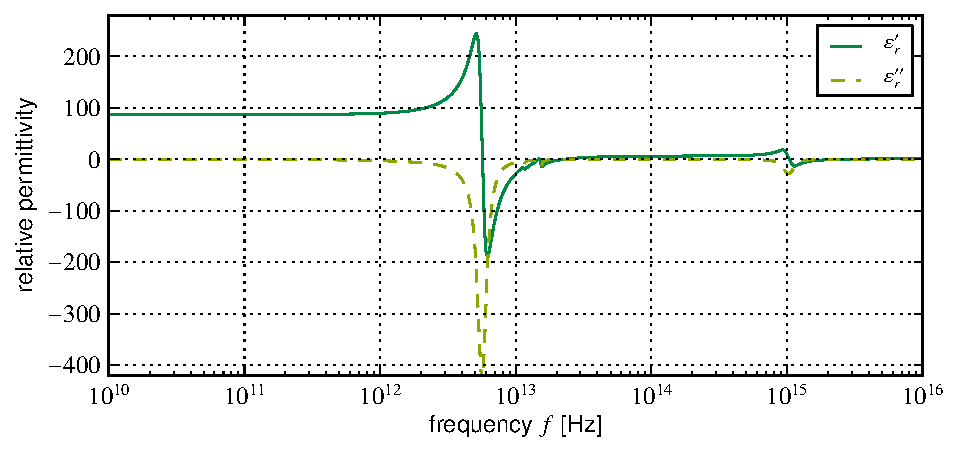
\includegraphics[width=14cm]{img/epsilon_TiO2_linear.pdf}
	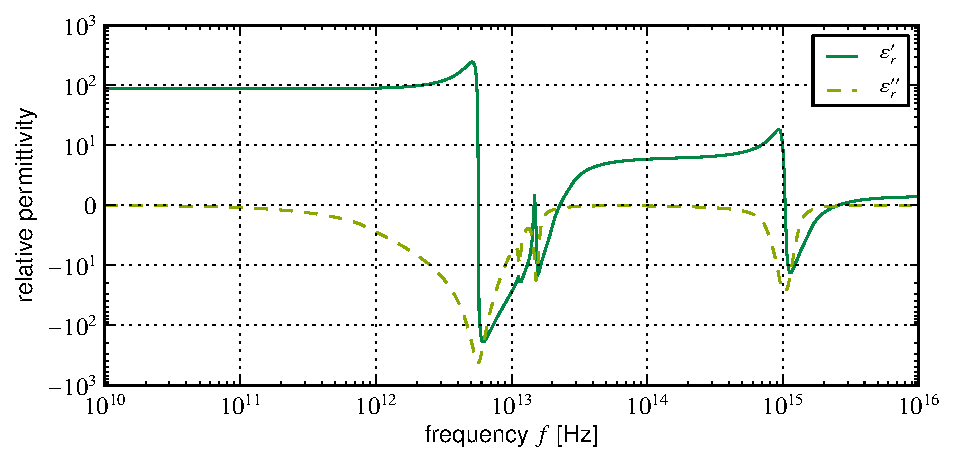
\includegraphics[width=14cm]{img/epsilon_TiO2_symlog.pdf}
\end{figure}


As described in Chapter \ref{chap_lorentzmedia}, the (local) response of usual media to an electromagnetic wave can be well approximated by a set of Lorentz oscillators, each of which is defined by three positive real numbers: its resonance angular frequency $\omega_{0m}$, damping rate $\gamma_m$ and oscillator strength $F_m$: % todo cite 
$$\hspace{3cm} \epsrl(\omega) = 1 + \sum_{m=1}^M \frac{F_m}{\omega_{0m}^2 - \omega^2 + \ii\omega\gamma_m} \hspace{3cm}\text{(\ref{eq_lorentz_eps} again)}$$
FDTD, being a time-domain method, requires the media to be described in a similar way with the difference that the nondispersive part of relative permittivity $\varepsilon_{r\infty}$ can be chosen as a real number. 
\begin{equation} \epsrl(\omega) = \varepsilon_{r\infty} + \sum_{m=1}^M \frac{F_m}{\omega_{0m}^2 - \omega^2 + \ii\omega\gamma_m} \label{eq_lorentz_eps_fdtd} \end{equation}
%It is not possible to directly supply the permittivity as an arbitrary function of frequency from fundamental reasons. 
%We thus return to the local Drude-Lorentz theory, with a due emphasis on the definition of materials in FDTD.
% we focus on this topic because in literature, either general theory is discussed, or just single working model  is used. We try to develop reliable rules for employing the FDTD to simulate realistic structures under as general circumstances as possible.


% TODO add a spectrum + table for SiO2?
%			or exp(-i omega t)					-> FFT has to be conjugated (??)




%}}}
\paragraph{Conditions of stability in FDTD}%{{{
%it was noted above that too high frequency of oscillators may introduce instability. 
%An important parameter is the critical frequency of the simulation, $f_c$ defined as 
% \begin{equation} f_c = \frac{c}{\pi \, C \, \Delta x},\label{eq_}\end{equation}
% where the \textit{Courant factor} $C$ is usually set to $C:=0.5$ and $c \approx 2.998 \cdot 10^8$ m/s is the speed of light. The voxel size thus determines the critical frequency; in a simulation typical for this thesis, $\Delta x := 2$ $\upmu$m and the critical frequency $f_c \approx 95$ THz lies in the mid-infrared. For simulations in visible range with $\Delta x := 50$ nm, and $f_c \approx 3800$ THz, that is, in the regime of hard UV radiation.

%The critical frequency may be viewed as the upper limit where an FDTD simulation gives plausible data. 
Author observed that $f_c$ determines the constraints for the simulation stability in two ways simultaneously:
\begin{enumerate}
 \item{The resonance frequencies must be below the critical frequency,  %% TODO get a proof, or some citation, or cite MEEP sources where S.G.Johnson wrote a routine about this
\begin{equation} \frac{\omega_{0m}}{2\pi} < f_c, \text{ for all oscillators, } \forall m \in \{1,2 \ldots M\}, \label{eq_fdtd_stability}\end{equation}
independent of what the strength $F_m$ or damping rate $\gamma_m$ of the oscillator is. 
%This relates to the above note about expressing all high-frequency oscillators in the form of the high-frequency (static) permittivity. . 
} 
 \item{The real part of the permittivity, as given in Eq. (\ref{eq_lorentz_eps_fdtd}), must be above a minimum value given by the Courant factor $S$ for all frequencies higher than the critical frequency $f_c$:
\begin{equation} \varepsilon_r'(2\pi\,f) > 3 S^{2} \equiv 3 \left( \frac{c \Delta t}{\Delta x} \right)^{2} \text{ for } \forall f \geq f_c. \label{eq_fdtd_stability_realp}\end{equation}  } % TODO verify whether the limit is eps>0 or e.g. eps>0.5 or whatever 
A geometrical interpretation of this rule is that the instability is introduced when any wave, of frequency above the critical frequency, can travel more than $1/\sqrt{3}$ of one FDTD cell size within one time step. 
Note that in a nonmagnetic medium, the traveled distance is $$\frac{c\Delta t}{\sqrt{\varepsilon_r'}}.$$
\end{enumerate}
The FDTD simulation will become unstable if one or both of these rules are broken. The error from the instability initially arises from inevitable numerical noise at the boundary of the problematic material and grows exponentially. It can be identified as a pixel-wise checkerboard pattern on the field snapshot. Later the field visualisation usually returns black images as the numerical infinity is reached within several tens of FDTD steps. 

\paragraph{Choice of the Courant factor}%{{{
Provided that a part of the simulation volume is empty vacuum with $\varepsilon_r'=1$, Eq. (\ref{eq_fdtd_stability_realp}) clearly determines the \textit{maximum value of Courant factor} 
$$S_{max} = 3^{-1/2}\approx0.577.$$
In practice, a slightly more conservative choice is made that provides a safe margin for the numerical imprecision: 
\begin{equation} S:= 0.500 \quad \rightarrow \quad \varepsilon_r'(2\pi\,f)> 0.75, \quad \forall f \geq f_c. \label{eq_courant_choice}\end{equation}
For any material with problematic high-frequency permittivity, $\varepsilon_r'(2\pi\,f_c) \in (0, 1)$, some low value of $S$ can be found that makes the simulation stable against the second rule. Simultaneously, the critical frequency shifts up, so potential problems with the first rule may be alleviated, too. This is however at the price of scaling up the number of required FDTD steps, so usually a reasonable change of the material definition is made instead of reducing $S$.

\add{
This is related to the \textit{Courant criterion} \cite{taflove2005book} that states for a nondispersive medium of permittivity $\varepsilon_r$ that 
$$\Delta t = S\,\frac{\Delta x}{c}  <  \frac{\sqrt{\varepsilon_r}}{\sqrt{3}}   \frac{\Delta x}{c}$$, as $S < n_{min}/\sqrt{dim}$ % TODO
i.e.
$$c \Delta t / n_{min} < \Delta x / \sqrt{dim} $$
which can be reformulated that   %TODO
}
%  /* Return true if the discretized Lorentzian ODE is intrinsically unstable,
%     i.e. if it corresponds to a filter with a pole z~outside the unit circle.
%     Note that the pole satisfies the quadratic equation:
%  			(z + 1/z - 2)/dt^2 + g*(z - 1/z)/(2*dt) + w^2 = 0
%     where w = 2*pi*omega_0 and g = 2*pi*gamma.   It is just a little
%     algebra from this to get the condition for a root with |z| > 1. */
%  static bool lorentzian_unstable(double omega_0, double gamma, double dt) {
%    double w = 2*pi*omega_0, g = 2*pi*gamma;
%    double g2 = g*dt/2, w2 = (w*dt)*(w*dt);
%    double b = (1 - w2/2) / (1 + g2), c = (1 - g2) / (1 + g2);
%    return b*b > c && 2*b*b - c + 2*fabs(b)*sqrt(b*b - c) > 1;
%  }
%}}}


%The first rule of $\omega_0/2\pi < f_c$ was observed to be very strict
%}}}
\paragraph{Practical aspects of material definition} %{{{
In all realistic media, the frequencies of different oscillators span over many orders of magnitude, and an accurate medium model would need to determine tens or hundreds of oscillators. Not all oscillators should be defined for a given FDTD simulation, however. 

\begin{figure}[t] \caption{Permittivity plot for titanium dioxide, similar to Fig. \ref{fg_tio2eps}. 
%Compared to the exact model of permittivity (green line), the model with reduced number of Lorentz oscillators was plotted (black line). 
The region forbidden by the stability rule is yellow shaded (above $f_c = 95$ THz and below $\varepsilon_r < 0.75$). The exact model for TiO$_{2}$ (green line) would be definitely unstable due to violating both stability conditions. The numerically stable model for frequency range of interest up to ca. 10 THz (black line) has all high-frequency oscillators substituted by increasing the value of $\varepsilon_{r\infty}$. Solid and dashed lines are real and imaginary parts, respectively. } \label{fg_tio2eps_stripped} \centering 
	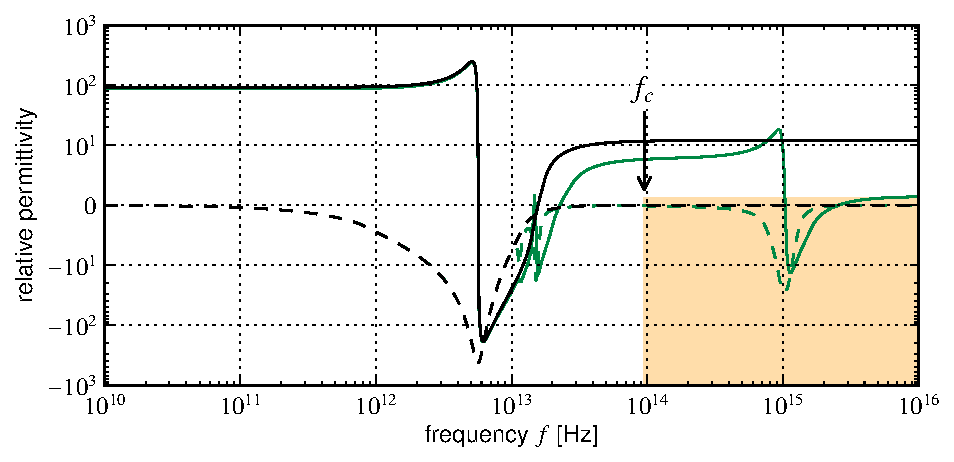
\includegraphics[width=14cm]{img/epsilon_TiO2stripped_symlog.pdf}
% full:
      % self.eps = 1
      % self.pol = [
      %         {'omega':5.67e12, 'gamma':1.05e12, 'sigma':50+90*extraordinary},      
      %         {'omega':11.43e12, 'gamma':.495e12, 'sigma':0.9*extraordinary},            
      %         {'omega':15.24e12, 'gamma':.72e12, 'sigma':2.6*extraordinary},            
      %         {'omega':1.0e15, 'gamma':.15e15, 'sigma':2.8 + .5*extraordinary},     ## imprecise two-Lorentzian approximation in UV
      %         {'omega':1.08e15, 'gamma':.15e15, 'sigma':2 + .4*extraordinary}            
% reduced: self.eps = 12.  self.pol = [ {'omega':5.67e12, 'gamma':1.05e12, 'sigma':50+30.} ]
\end{figure}

First of all, high-frequency oscillators would make the simulation unstable.
Aside from this, adding overly many oscillators is also inefficient, because each oscillator defined increases computing difficulty in FDTD. 
It is therefore advisable to weed the oscillators to a minimum acceptable number necessary, and to describe the material within some frequency range of interest (FRoI) % TODO  define range of interest
only:
\begin{enumerate}
 \item{
%Often the first step in processing FDTD results lies in converting them to frequency domain via Fourier transform. 
The upper bound for FRoI is limited by numerical stability as stated above. Mostly, a more strict limit is given by the spatial resolution of the simulation: In a high-permittivity material, high frequencies correspond to wavelengths similar to the voxel size (or even smaller than it), leading to significant inaccuracy. 

Each oscillator far above the frequency of interest shall be expressed only as a constant added to the nondispersive part of permittivity $\varepsilon_{r\infty}$. This contribution is given by Eq. (\ref{eq_delta_eps}) as 
$$\Delta \varepsilon_r = \frac{F}{\omega_0^2}.$$ 
If some of the high-frequency oscillators introduces significant dispersion or losses in the FRoI, it it should not be eliminated this way. This usually concerns the oscillator that is the closest above FRoI, and it usually can be maintained without causing instability.
} 
 \item{
Very low frequencies, corresponding to wavelengths much greater than the whole simulation volume, are theoretically accessible with a long-enough FDTD simulation, but the FRoI usually does not reach zero frequency, mostly for practical reasons. If needed, the low-frequency phenomena can often be computed more efficiently in a separate simulation with a lower resolution or even with different numerical methods.

The oscillators at frequencies too low can therefore be omitted without any change to the behaviour within the FRoI. One important exception is the low-frequency oscillator that defines conductive behaviour, as described below.
} 
 \end{enumerate}
%}}}

\paragraph{Drude model for conductive media} %{{{
The Drude model assumes the relative permittivity in the form
\begin{equation} \epsr(\omega) = 1 + \frac{\omega_p^{2}}{0 - \omega^{2} + \ii\gamma\omega} = 1 - \frac{\omega_p^{2}}{\omega^{2} - \ii\gamma\omega}, \label{eq_drude_eps}\end{equation}
where $\omega_p$ and $\gamma$ are two independent parameters that describe the metal: 
\begin{itemize}
 \item{$\omega_p$ is the \textit{plasma frequency}, at which the real part of permittivity crosses zero. The physical consequence is that for $\omega > \omega_p$ the medium allows the transverse electromagnetic wave to propagate through. 
%The angular frequency of $\omega_p$, the longitudinal (electric) waves oscillate. 
%The quasiparticle associated with the oscillation of the charge in bulk conductive medium, a \textit{plasmon}, has given the name to $\omega_p$. % TODO add a relation to the chapter on "dispersion in local media"
 } 
 \item{$\gamma$ maintains its meaning as the \textit{rate of exponential decay} of the medium response to an impulse. The Drude model was conceived in the early 20th century, with the simplified hypothesis that electrons would be freely propagating particles that undergo collisions with the atoms at an average frequency $\gamma$. Upon the colision, their speed would either drop to zero, or (equivalently) would be randomized. Although the mechanism of resistivity is more complicated than this, the parameter $\gamma$ is commonly denoted as the \textit{scattering frequency}.} 
 \end{itemize}
%Both have the dimension of $\mathrm{rad\; s^{-1}}$. 
The Drude model can thus be considered a specific case of a Lorentz oscillator with $\omega_0 = 0$, and oscillator strength given by $F = \omega_p^2$. 
Obviously, using Eq. (\ref{eq_delta_eps}) to compute the contribution of the Drude term to the real part of permittivity would give infinite values, as static electric field can displace unlimited amount of charge in a conductor.

If $\gamma$ is nonzero, the permittivity is a complex function and it can be separated into its real and imaginary part $\varepsilon_r = \varepsilon_r'+\ii\varepsilon_r''$ by expanding the fraction in (\ref{eq_drude_eps}) by complex conjugate of its denominator
\begin{equation} \varepsilon_r = 1 - \omega_p^{2} \cdot \frac{\omega^{2} + \ii \gamma \omega}{\omega^{4} + \gamma^{2} \omega^{2}} = 
		\underbrace{\left(1 - \frac{\omega_p^2}{\omega^2+\gamma^2}\right) }_{\text{real part } \varepsilon_r'}
+ \ii	\underbrace{\left(\frac{-\omega_p^2\gamma}{\omega^3 + \gamma^2\omega}\right) }_{\text{imaginary part } \varepsilon_r''}.
\label{eq_drude_eps_loss}\end{equation}
%The real part $\varepsilon_r'$ indicates capacitive or reactive behaviour of the metal. The imaginary part $\varepsilon_r''$ describes losses which may arise either from 
% \underbrace{ }_{\text{}}
The low- and high-frequency limits of permittivity given by the Drude model are:
\begin{equation} \lim_{\omega \to 0} \varepsilon_r' = 1-\frac{\omega_p^2}{\gamma^2}, \quad \quad  
				 \lim_{\omega \to 0} (\varepsilon_r'' \cdot \omega) = -\frac{\omega_p^2}{\gamma},\label{eq_drude_limlow}\end{equation}
\begin{equation} \lim_{\omega \to +\infty} \varepsilon_r' = 1, \quad \quad  
				 \lim_{\omega \to +\infty} (\varepsilon_r'' \cdot \omega^3) = -\omega_p^2 \gamma. \label{eq_drude_limup}\end{equation}
We can see that in the low frequency limit, the imaginary part of permittivity diverges (while its real part has a finite value). In the high frequency limit, the metal permittivity approaches that of vacuum, i.e. $1+0\ii$.
%}}}
\label{chap_fdtd_drude}
\paragraph{Low- and high-frequency limits of conductivity in the Drude model}%{{{
The notion of \textit{conductivity} is widely used to describe metals and doped semiconductors, i.e. media where the response to the electric field is characteristic by the motion of free charge carriers. 
Generally, both permittivity $\varepsilon_r(\omega)$ and conductivity $\sigma(\omega)$ are complex functions of the angular frequency $\omega$. As long as the approximation of negligible spatial dispersion is used, each of them is fully determined by the other function. % maybe even if spatial dispersion is nonzero -> check this?
For clarity, we avoid using the conductivity in the rest of the thesis except this chapter.

The relation between $\varepsilon_r(\omega)$ and $\sigma(\omega)$
 can be derived by realizing that the current in a material is always caused by movement of charges with density $\rho$ and average velocity $\mathbf{v}(t)$. The conduction and polarisation currents are not distinguished here, as their density is given as $\rho \mathbf{v}(t)$ in both cases. When current is excited by a harmonic electric field $E(t) = \mathrm{e}^{\ii\omega t}$: %TODO FIXME explain rho.n, use i omega t instead of -i omega t, check again...
\begin{equation} \rho \mathbf{v}(t) = \sigma(\omega) E(t) = \sigma(\omega) \mathrm{e}^{\ii\omega t}, \quad\text{ (conduction approach -- Ohm law)} \label{eq_rho_n1}\end{equation}
\begin{equation} \rho \mathbf{v}(t) = \varepsilon_0 \varepsilon_r(\omega) \frac{\partial E(t)}{\partial t} = \ii \omega \varepsilon_0 \varepsilon_r(\omega) \mathrm{e}^{\ii\omega t} . \quad\text{ (displacement current approach)} \label{eq_rho_n2}\end{equation}
Both above equations describe the same quantity, so
\begin{equation} \sigma(\omega) = \ii \omega \varepsilon_0 \varepsilon_r(\omega), \quad  \text{and} \quad  \varepsilon_r(\omega)  = \frac{\sigma(\omega)}{\ii \omega \varepsilon_0}. \label{eq_drude_sigma}\end{equation}
Thus, a dielectric medium with real constant permittivity has \textit{imaginary} conductivity, magnitude of which grows with frequency (cf. the admittance of a capacitor). A conductor with real constant conductivity has complex permittivity, and its imaginary part diverges in the low-frequency limit. 

\begin{figure}[t] \caption{Permittivity and conductivity plot for gold; vertical scale and the yellow region forbidden by the stability rules are the same as in Fig. \ref{fg_tio2eps_stripped}. The exact model of gold % TODO \cite{palik} 
(red) is compared to the lossy Drude model with Lorentz oscillators substituted by $\varepsilon_r$ (blue), and for illustration, also to the lossless Drude model with scattering frequency set to zero (grey). Obviously, none of these models is numerically stable if $f_c = 95$ THz.
\\The bottom plot shows the conductivity of these three models as given by Eq. (\ref{eq_drude_sigma}).}
\label{fg_Au_models} \centering 
	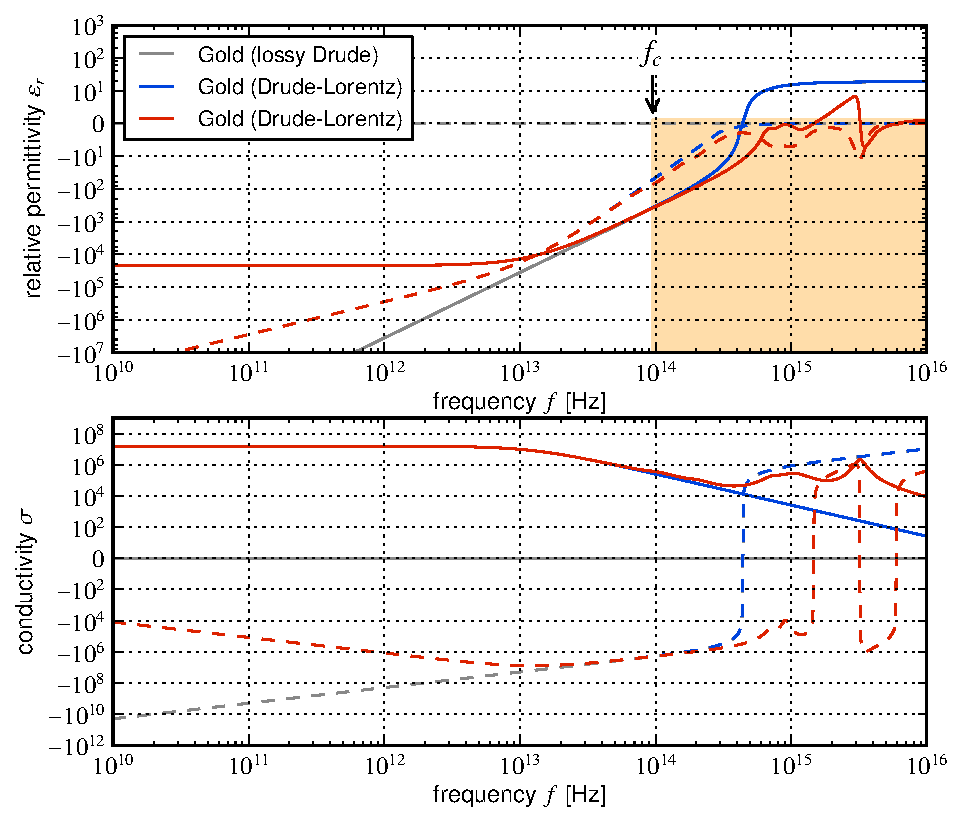
\includegraphics[width=14cm]{img/epsilon_Au_models_llgrey.pdf} % Scattering freq of gold = 12.8 THz
\end{figure}


Using the above relation (\ref{eq_drude_sigma}) to convert metal permittivity $\varepsilon_r(\omega)$ into conductivity $\sigma(\omega)$, and substituting the Drude-model permittivity (\ref{eq_drude_eps_loss}), we obtain
\begin{equation} \sigma(\omega) = \ii \omega \varepsilon_0 \varepsilon_r(\omega)= \ii\omega \varepsilon_0 \varepsilon_r'(\omega)  -  \omega \varepsilon_0 \varepsilon_r''(\omega) = 
	\ii \underbrace{\varepsilon_0 \left(\omega - \frac{\omega_p^2\omega}{\omega^2+\gamma^2}\right)}_{\text{imaginary part } \sigma''}  + 
		\underbrace{\varepsilon_0\frac{\omega_p^2\gamma}{\omega^2+\gamma^2}}_{\text{real part } \sigma'}. \label{eq_drude_sigmaeps1}\end{equation}
We may now express the low- and high-frequency limits also for conductivity:
\begin{equation} \sigma_{LF} := \lim_{\omega \to 0} \sigma' = \frac{\omega_p^2\varepsilon_0}{\gamma}, \quad \quad  
				 \lim_{\omega \to 0} (\sigma'' / \omega) = \varepsilon_0 - \frac{\omega_p^2 \varepsilon_0}{\gamma^2} , \label{eq_drude_sigmalimlow}\end{equation}
\begin{equation} \lim_{\omega \to +\infty} (\sigma' \cdot \omega^2) = \varepsilon_0\omega_p^2\gamma, \quad \quad  
				 \lim_{\omega \to +\infty} (\sigma'' / \omega) = \varepsilon_0. \label{eq_drude_sigma_limup}\end{equation}
Let us note again that in the literature that uses the negative phase convention $e^{-\ii \omega t}$, the resulting $\varepsilon_r(\omega)$ and $\sigma(\omega)$ are complex conjugated to the results above. 
%}}}

\paragraph{Defining resistive metals for stable low-resolution simulations} %{{{
Simulations in the optical range are relatively safe in terms of numerical stability. From Eq. (\ref{eq_fc}) it follows that the resolution of $\Delta x = 50$ nm, suitable for NIR/visible spectrum, yields the critical frequency $f_c = 3.82\cdot 10^{15}$ Hz ($\lambda = c/f_c \approx 78$ nm), which is far above the plasma frequency of metals or other conductors. Accordingly, no changes are usually needed to be made in the Drude model, although the simulation may run faster if one or more Lorentz terms outside FRoI can be omitted.
%If high precision of the metal model is needed, one is also free to add one or more Lorentz oscillators in the optical/UV range to refine the shape of permittivity.
 
Realistic simulations of metals at lower resolutions however require taking measures to ensure stability, as the critical frequency $f_c$ is reduced below the plasma frequency of most metals when $\Delta x \gtrsim 200$ nm. % TODO check this
A trivial approach is to drastically reduce the Courant factor $S$ so that $f_c$ remains above plasma frequency. Although this should reliably avoid the instability, it would be so at the expense of scaling the computational time. As a general rule, lower resolution is typically chosen for larger structures, where also all investigated processes accordingly happen on a longer timescale.
%Drude model is known to introduce negative permittivity up to optical range, so 
%Assuming the critical frequency is far below the optical range, the Lorentz oscillators can be certainly neglected. Nonetheless, negative permittivity above critical frequency still introduces instability, which has to be resolved. 

For simulations with lower resolution, it is much more efficient to replace the exact Drude model with its approximation that maintains the same low-frequency limit of conductivity $\sigma_{LF}$, but has positive permittivity around the critical frequency and above it. 
This formally inverts the relations that describe the material:
\begin{itemize}
\item{
For \textit{high-resolution simulations}, $\omega_p$ and $\gamma$ are given as experimental properties of the metal, while $\sigma_{LF} = \omega_p^2\varepsilon_0\gamma^{-1}$ is determined by them and the nondispersive part of permittivity $\varepsilon_{r\infty} = 1$ is fixed to that of vacuum. 
} 
\item{
For \textit{low-resolution simulations}, the situation is opposite: $\sigma_{LF}$ is given as one experimental property, $\gamma < 2\pi f_c$ is given by the critical frequency, % TODO describe why so
whereas $\varepsilon_{r\infty}$ and $\omega_p$ are to be determined from the previous two input parameters.
} 
\end{itemize}
In this section we develop the strategy to determine the correct combinations of  $\gamma < 2\pi f_c$, $\varepsilon_{r\infty}$ and $\omega_p$.

\add{

%The value of $\gamma$ is also limited to be lower than $2\pi f_c$, so its value is fixed to be as close to $2\pi f_c$ as possible. % TODO ...is it? verify and add to the rules for stability written above
The values of the plasma frequency $\omega_p$ as well as the  $\varepsilon_{r\infty}$ remain to be freely manipulated.

        $$ \gamma = 2\pi f_c \cdot gammafactor $$
        % test when unstable -> reduce self.gamma by 100 -> test again -> finally write automatic selection of value

        % Knowing the scattering frequency gamma, the virtual plasma frequency is now determined by lfconductivity
        $$ \omega_p = \sqrt{\frac{\gamma \sigma_{LF}}{\varepsilon_0}} $$

        % The following step is required for FDTD stability: 
        % Add such an high-frequency-epsilon value that shifts the permittivity to be positive at f_c
        % If self.eps>1, the frequency where permittivity goes positive will generally be less than f_p
        $$\varepsilon_{r\infty} = (\omega_p/(2\pi f_c))^2 \text{ or 1 if it would be lower} $$
}

%}}}
\paragraph{Conductive media in FDTD} %{{{
The resonance frequency $\omega_0$ is inversely proportional to the square root of the restoring force in the harmonic oscillator. A conductive medium is characteristic by having part of the charges that do not experience any restoring force, so they can be modelled by an oscillator with a resonance frequency approaching zero: $\omega_0 \rightarrow 0$; in practice any value lower than the inverse of simulation time gives expected results.

%When $\omega_0$ is reduced to small values, the oscillator epsilon difference $\Sigma = \Delta \varepsilon_r$ has to be upscaled accordingly to keep the plasma frequency constant.
%When $\omega_0$ is reduced to small values, the oscillator strength $F$ shall be kept constant?



%% TODO should not describe the lorentz-drude model here -> this is to be done it the Theory section
%}}}
\paragraph{Debye media in FDTD} \label{fdtd_debye} %{{{
The Lorentz model can be employed also to define overdamped oscillators, corresponding to the processes where  $\gamma \gg \omega_0$, i.e. the inertia is negligible.
A typical example is the  reorientation of polar molecules in liquids or solids. 

It can be shown that for $\gamma \gg \omega_0$, the peak of $\varepsilon_r''(\omega)$ lies approximately on the frequency $\omega_p^{2}/\gamma$. The spectral width of such a peak is proportional to its central frequency. 

% TODO figure illustrating this

\begin{table}[ht]   \caption{}  \label{tb_} \centering 
\begin{tabular}{cc|cc}
 \toprule
\textbf{Charges are}	& \textbf{Inertia is}				& \textbf{Phenomenon}				& \textbf{Example}		 \\
 \hline
Bounded		& Significant				& Lorentz oscillator					& \shortstack{optical phonons, \\electronic levels,\\ molecular vibration \\or rotation in gases}	\\
 \hline
Bounded		& Negligible				& Debye relaxation						& \shortstack{molecular rotation \\in solids or liquids} \\
 \hline
Unbounded	& Significant				& \shortstack{Reactive\\(plasmonic) medium}			& \shortstack{colisionless plasma, \\metals (from mid-infrared\\to optical range)} \\
 \hline
Unbounded	& Negligible				& Resistive medium						& \shortstack{doped semiconductors,\\\newline metals (in far-infrared\\ range and below)} \\
 \bottomrule
 \end{tabular} \end{table}


%}}}
\paragraph{Selection of FDTD implementations} %{{{
MEEP, OpenEMS, B-Calm, EMTL, 
%}}}
\paragraph{} %{{{
%}}}
\paragraph{} %{{{
%}}}
\subsection{Plane-wave expansion method} % TODO
\subsection{Transfer-matrix method} % TODO
%illustrates the band-gap formation \cite{laktionov2008}

\subsection{Filter-diagonalisation method} % TODO

\section{Simulation setups for metamaterial homogenization} % TODO
\subsection{Scattering parameters} % TODO
\paragraph{Simulation geometry} %{{{
\begin{figure} \caption{geometry}  \centering 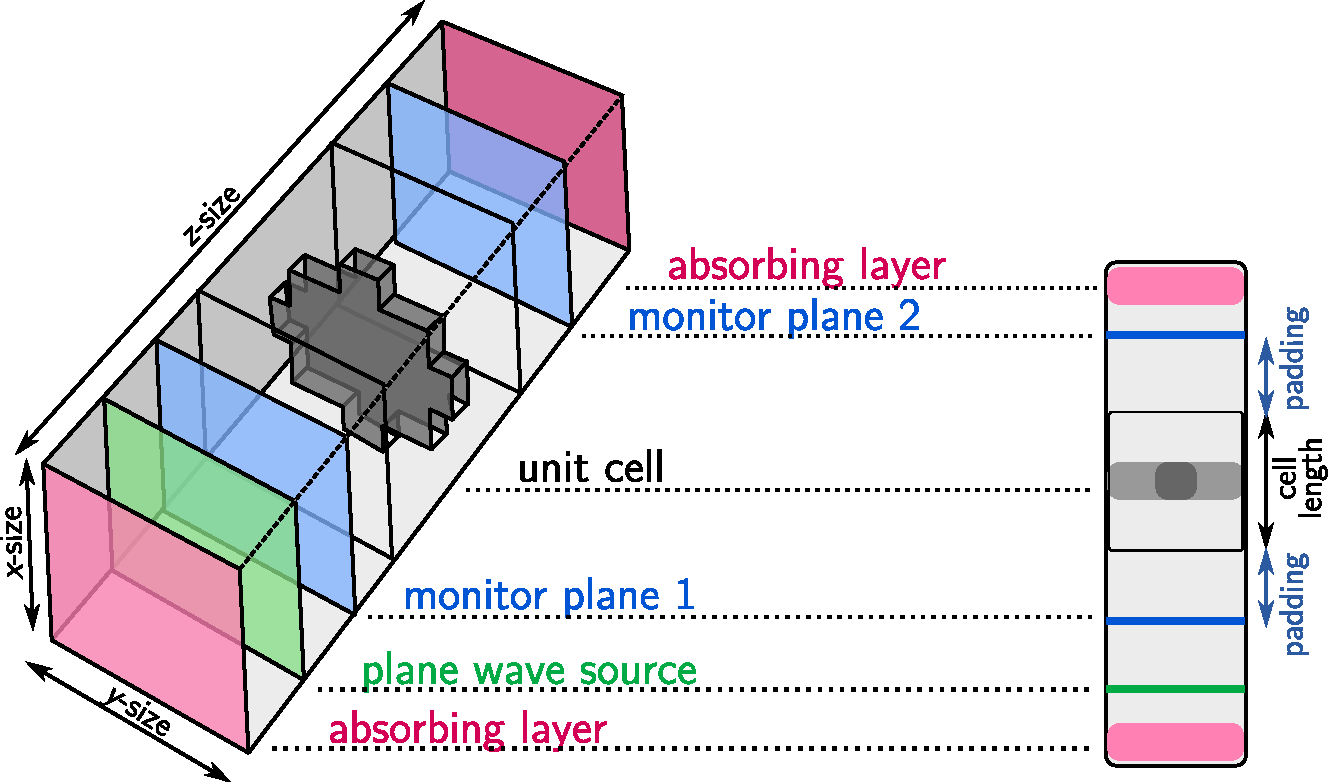
\includegraphics[width=10cm]{img/meep_geometry.pdf} \end{figure} \clearpage
%% (in fact, this is independent of FDTD, only to the time-marching methods)
%% \cite{terao2011}
%}}}
\paragraph{Avoiding detection of near-field in monitor planes} %{{{
%% Hynek's trick
%}}}
\paragraph{} %{{{
%}}}
\paragraph{Effective-parameter retrieval by smith2002} %{{{

\begin{figure} \caption{1red.pdf}  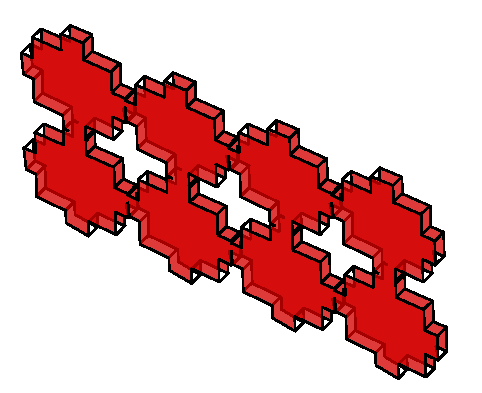
\includegraphics[width=3cm]{img/multilay_1red.pdf}
               \caption{2gn.pdf}   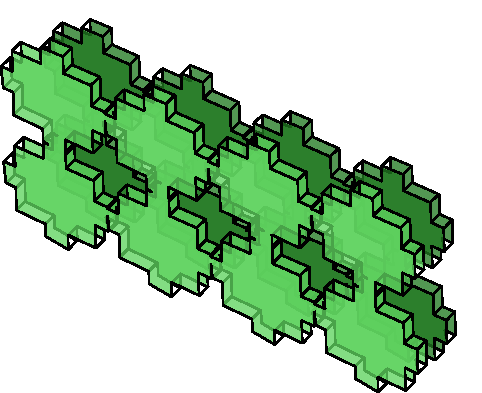
\includegraphics[width=3cm]{img/multilay_2gn.pdf}
               \caption{3bu.pdf}   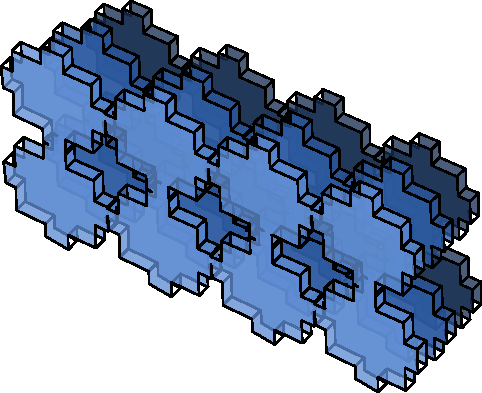
\includegraphics[width=3cm]{img/multilay_3bu.pdf}
               \caption{3grey.pdf} 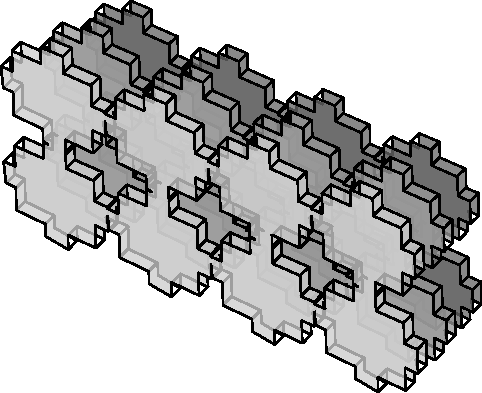
\includegraphics[width=3cm]{img/multilay_3grey.pdf}
               \caption{4vio.pdf}  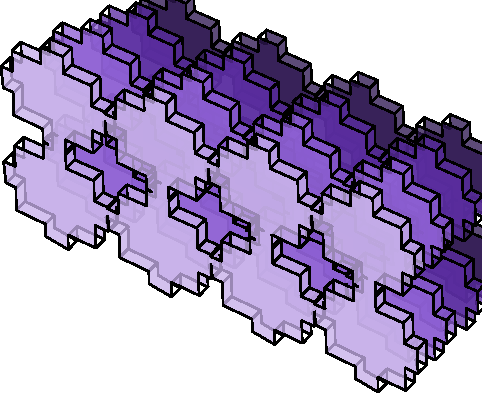
\includegraphics[width=3cm]{img/multilay_4vio.pdf} \end{figure} \clearpage
%}}}
\paragraph{Unambiguous arccosine} %{{{
%See ~/p/MEEP_2013/130711_EWires/19_TiO2_cellscan_thick_HR/
\begin{figure} \caption{new}  \centering 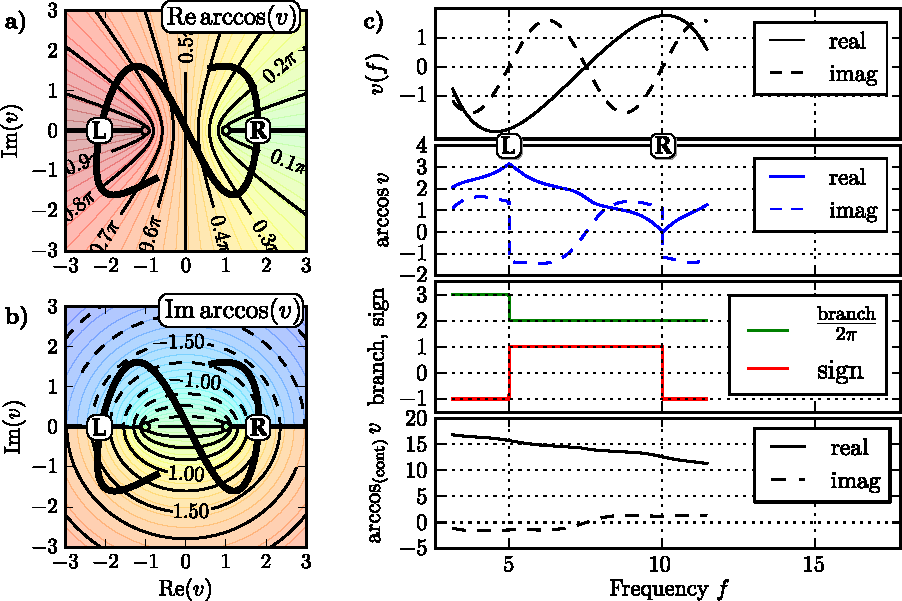
\includegraphics[width=\textwidth]{img/continuous_arccos/continuous_arccos_new.pdf}  \end{figure}\clearpage
%}}}
\subsection{Current-driven homogenisation} % TODO
\begin{figure} \caption{img/cdh\_srrwire\_structure.pdf}  \centering 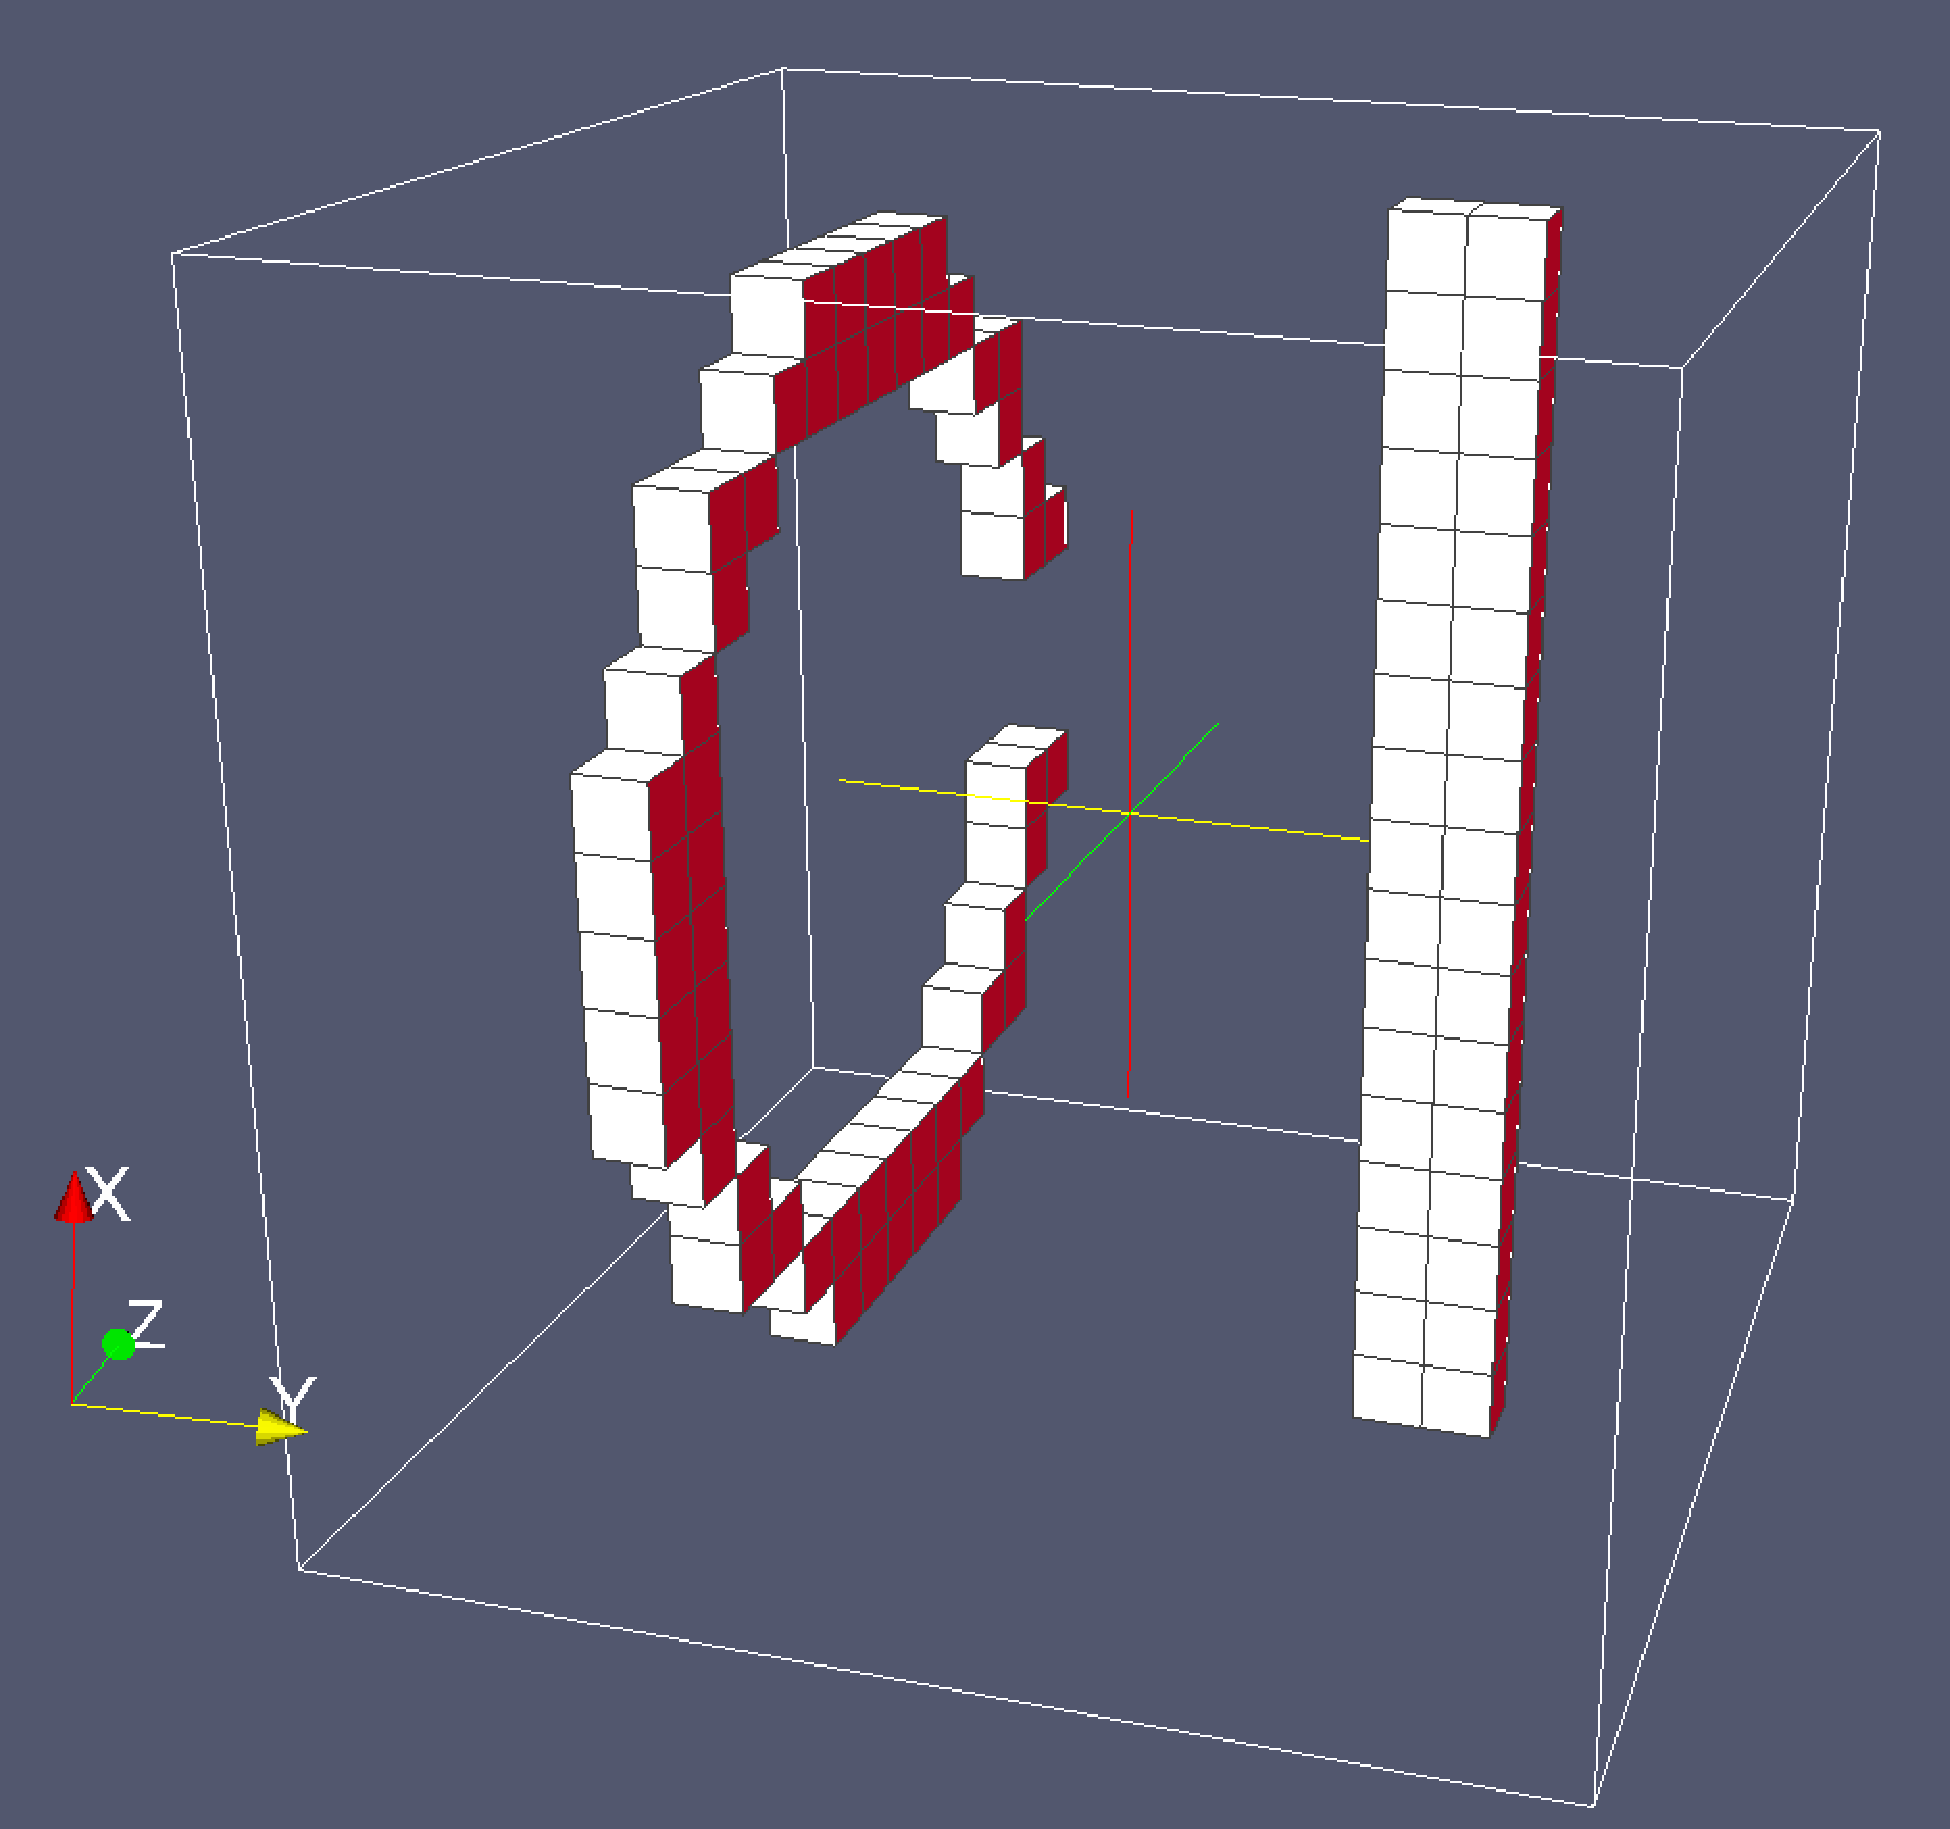
\includegraphics[width=10cm]{img/cdh_srrwire_structure.pdf} \end{figure} \clearpage
\begin{figure} \caption{img/cdh\_srrwirethick.pdf}  \centering 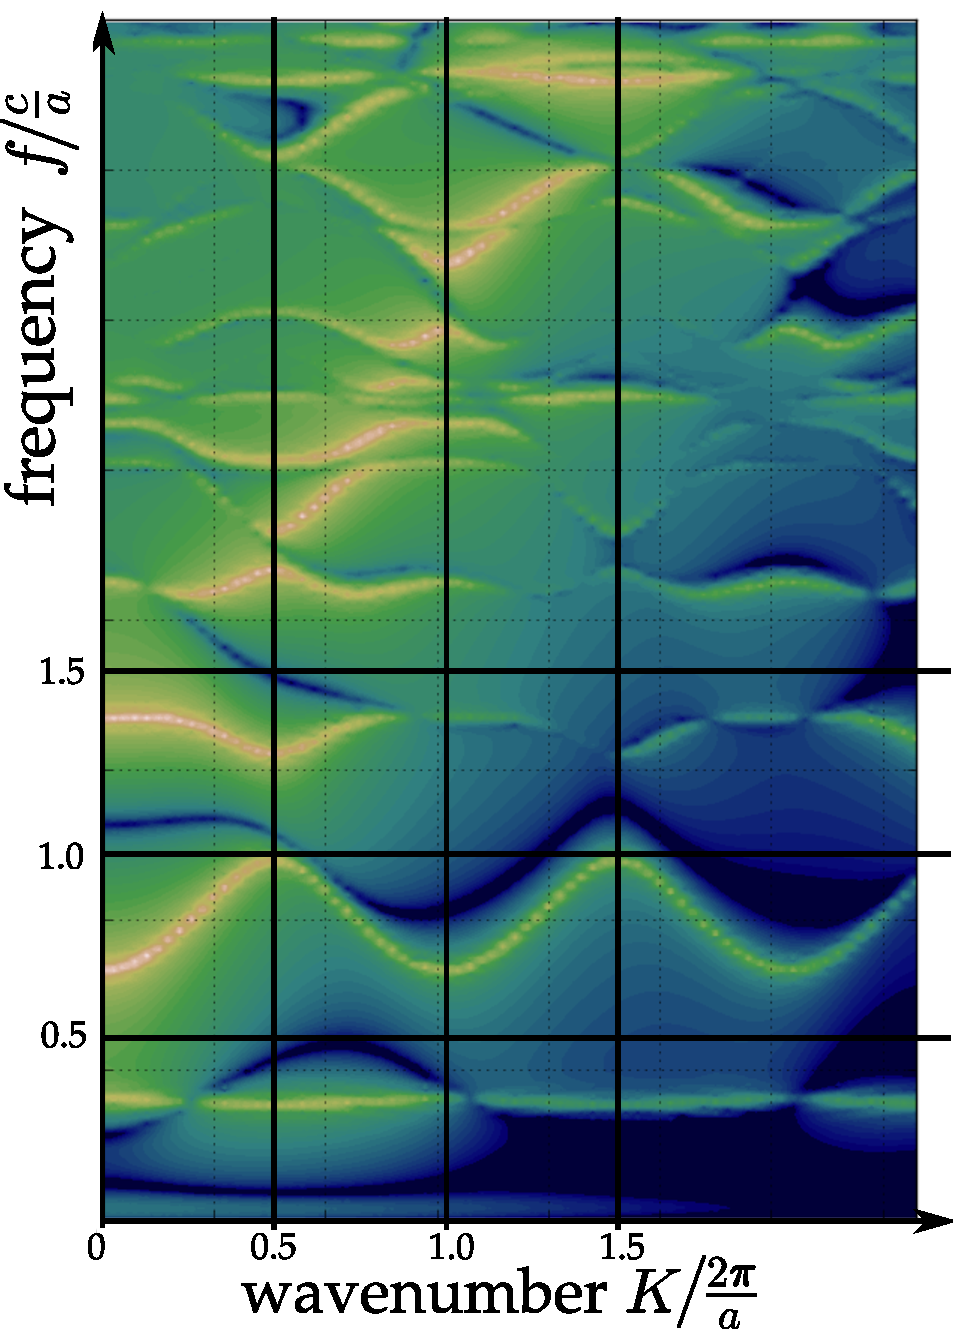
\includegraphics[width=10cm]{img/cdh_srrwirethick.pdf} \end{figure} \clearpage
\subsection{Simulation of refraction on a wedge} % TODO

\section{Terahertz experiments} % TODO
\begin{figure} \caption{img/exp\_THz\_sampling.pdf}  \centering 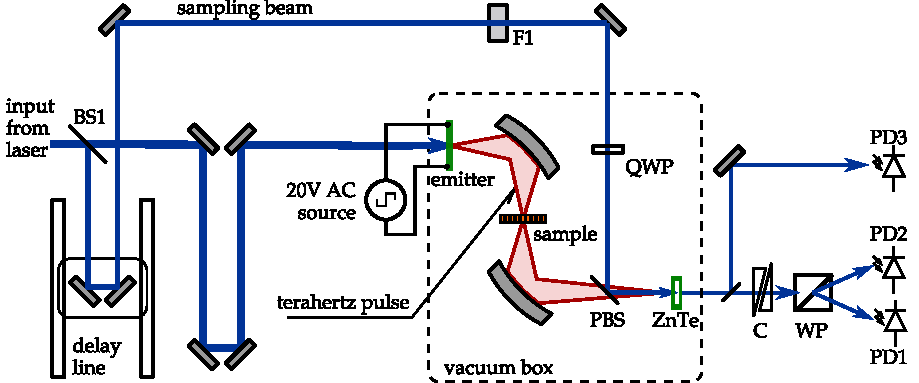
\includegraphics[width=10cm]{img/exp_THz_sampling.pdf} \end{figure} \clearpage
\subsection{Terahertz generation and detection setup}%{{{
The numerical data could be in some cases corroborated by experimental measurement using the \textit{time-domain terahertz spectroscopy} (TDTS) in our laboratory. 

The approach is similar to that used in the FDTD simulations. A short, broadband pulse impinges the sample, one part of its energy is transmitted, another reflected and the rest is absorbed in the sample. The transmitted pulse is then recorded by the time-domain sampling setup. The resulting transmission is computed by means of Fourier transform as a complex spectrum, which is to be normalized by the spectrum of the incident pulse.

%The experimental geometry is somewhat similar to that used for FDTD simulations above. Also the results are similar: we get the complex amplitude transmission spectrum,  
\begin{figure}[ht] \caption{\textit{Experimental setup for terahertz time-domain spectroscopy}} \label{fg_exp} \centering 
	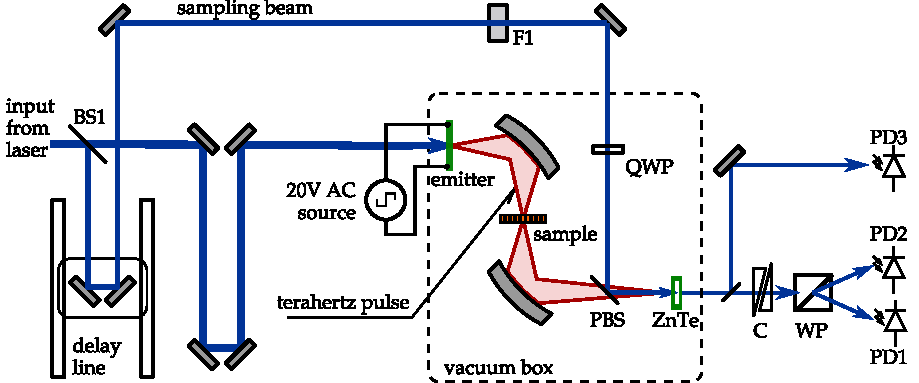
\includegraphics[width=12cm]{img/exp_THz_sampling.pdf}
\end{figure}

The crucial component of the terahertz generation and detection setup is a source of ultrashort optical pulses. We used \textit{Coherent Mira} femtosecond oscillator with mean power of 0.5 W, central wavelength 810 nm,  and a pulse duration under 70 fs. The optical pulses are split at beamsplitter (BS1) into the \textit{probe} branch and the \textit{sampling} branch. 
\begin{itemize}
 \item{The probe branch passed through a mechanical chopper, which is needed for synchronous detection, and impinged a terahertz emitter. The emitter, a biased interdigitated antenna on a fast-switching semiconductor, responds to an optical pulse by fast discharging and emitting of a broadband electromagnetic pulse with spectral components from 100 GHz to 3 THz. This pulse, denoted by red area to indicate its diffractive nature, passes through the sample under study followed by a pellicle beamsplitter (PBS) and finally impinges a ZnTe nonlinear crystal. } 
 \item{The \textit{sampling} branch reflects from a pair of mirrors on a delay line, acquiring a precisely controlled relative delay against the first branch. Then it is properly attenuated at filter (F1) and its polarisation is converted from linear to a circular one on a quarter-wave plate (QWP). The pellicle beamsplitter directs the optical beam along the axis of the terahertz beam.} 
 \end{itemize}
%% TODO add references to other papers and theses from our group - one can not describe everything from Gouy shift to PKGraph ...
%}}}
\subsection{Scheme for simultaneous measurement of reflection and transmission}%{{{
It is theoretically possible to measure the \textit{reflection spectrum} using TDTS in a similar way the transmission spectrum was measured. However, due to the complexity of such a setup and sensitivity to sample displacement, we did not use a second sampling branch for reflected signal. Instead of using two sampling schemes, it is possible to recover the amplitude and phase reflectivity of a sample by stacking it between a pair of thick (3 and 6 mm) sapphire slabs. Thanks to the relatively high refractive index of sapphire ($N \approx 3.4$), these slabs introduce several distinct  echoes into the transmission signal.

\begin{figure} \caption{A broadband pulse passes through a single layer of microspheres randomly arranged between two sapphire slabs and is sampled by electrooptical detection.}  \centering 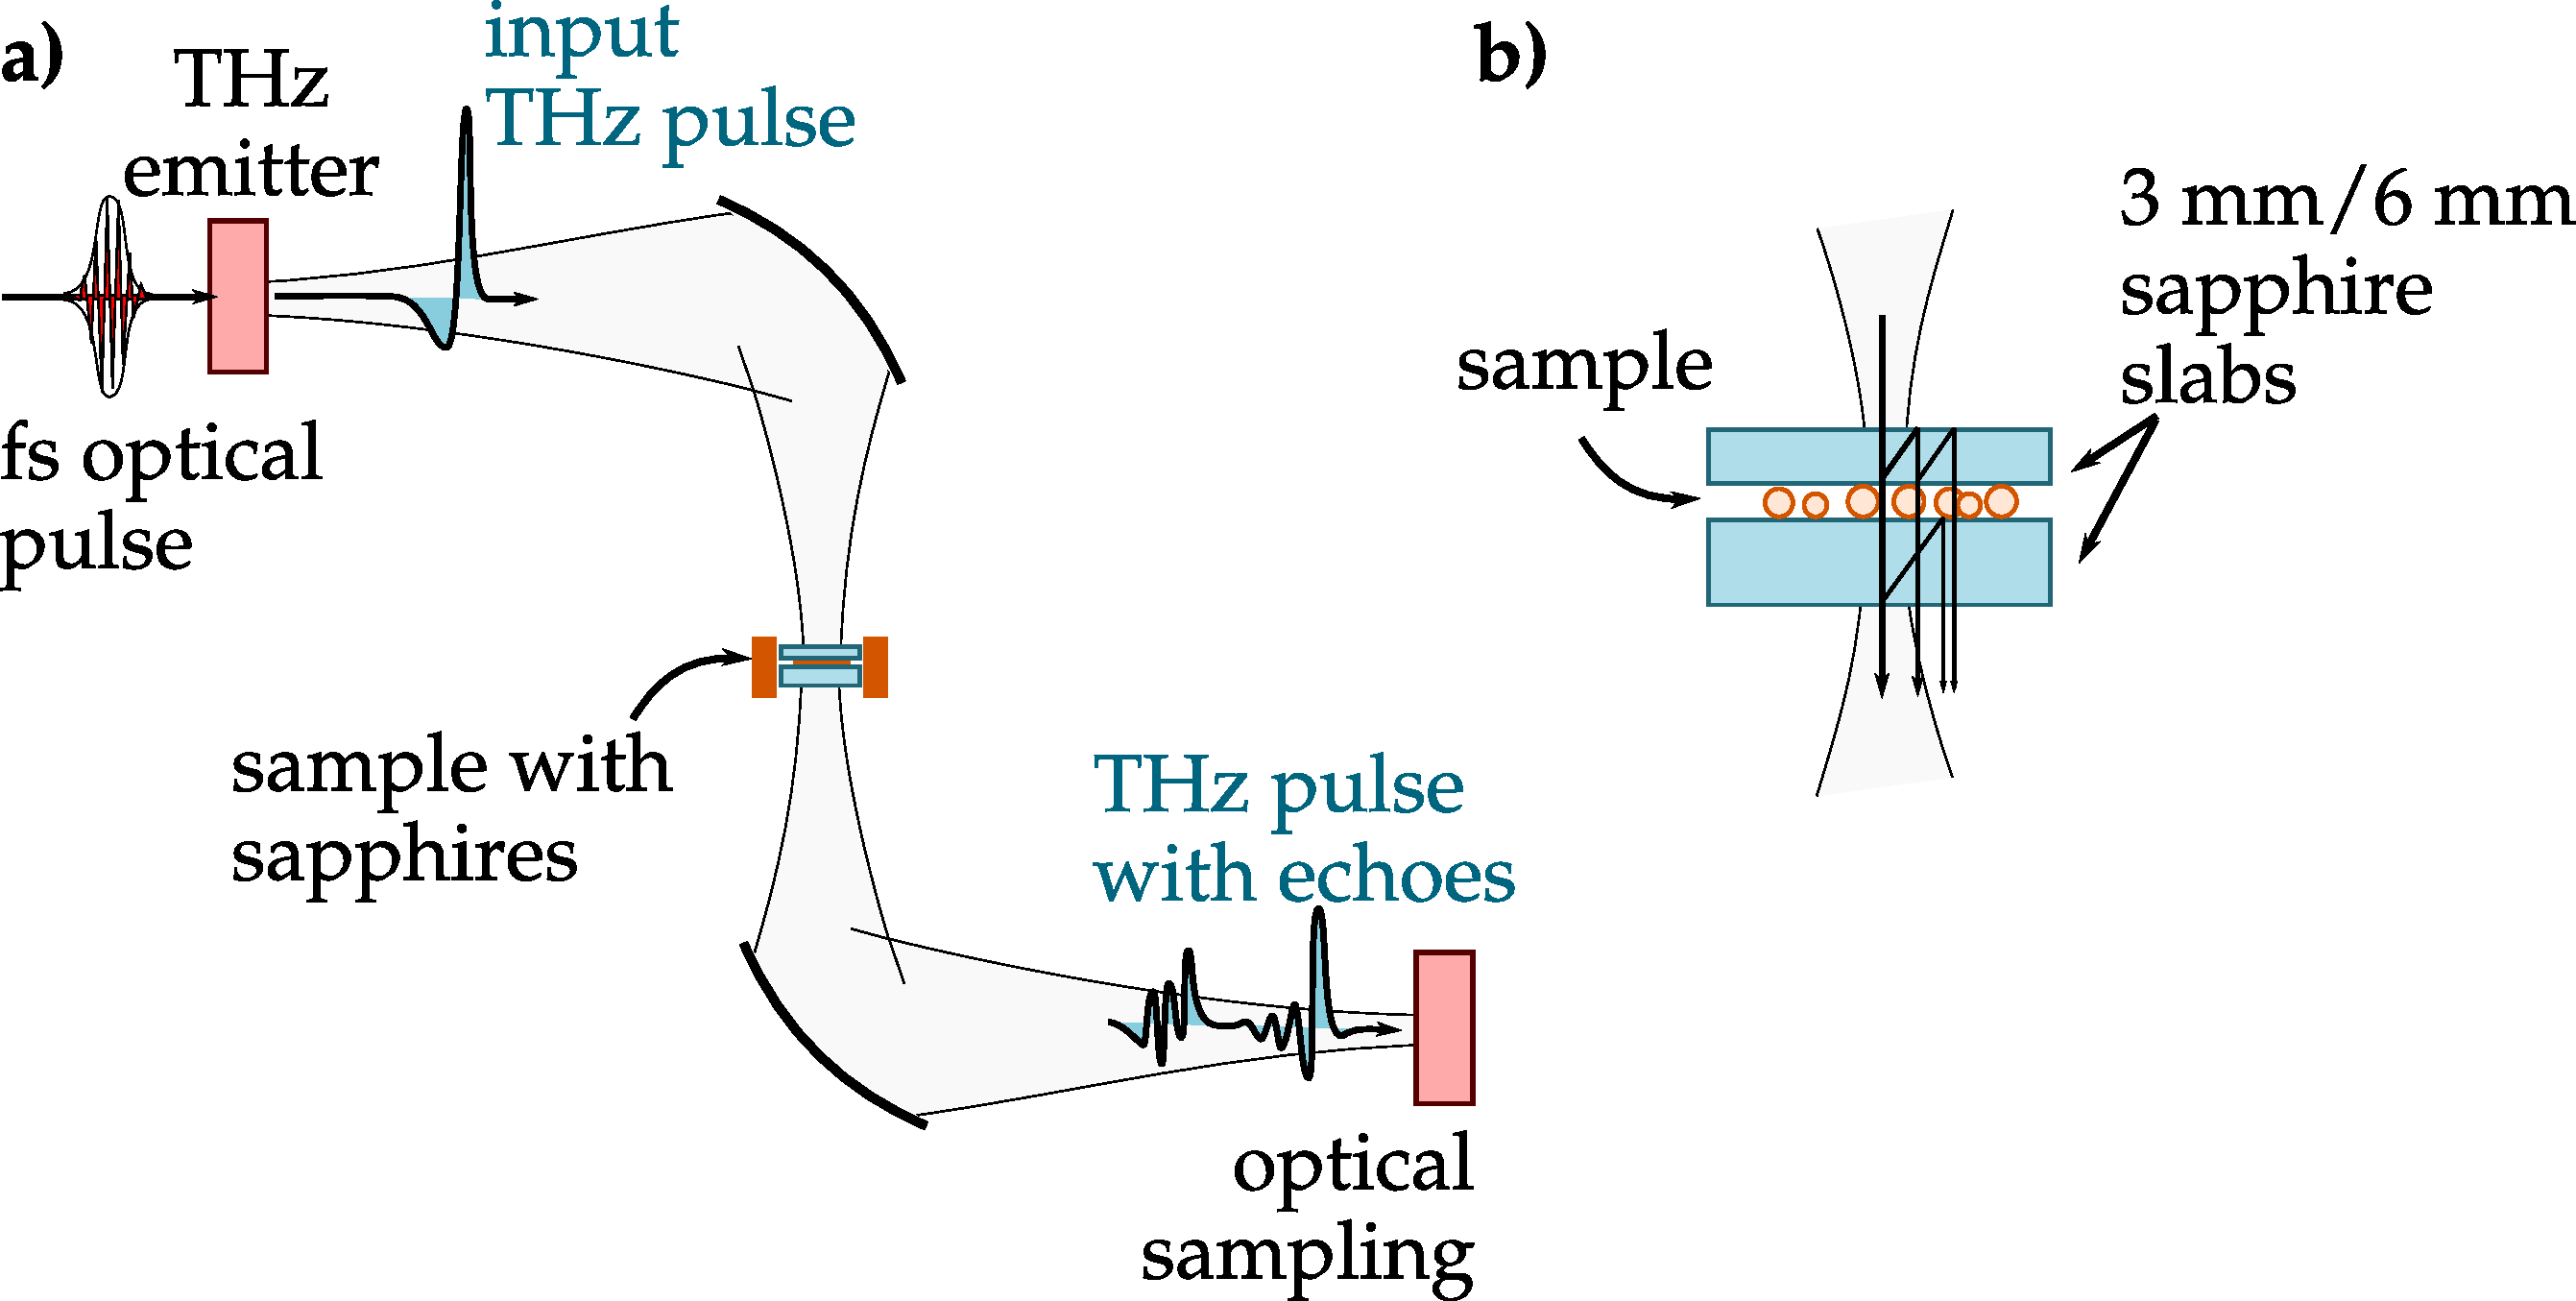
\includegraphics[width=12cm]{img/expe/sample_sapphires.pdf} \end{figure} \clearpage

If the beam divergence is neglected, each optical element can be characterised by its complex transfer function in the resulting spectrum. One needs to define three transmission functions for the beam passing the volume of the thin sapphire $A(f)$, thick sapphire $B(f)$ and of the sample $t(f)$, and two reflection functions for the beam reflected on sapphire-air interface $r_{A}(f)$ and on the sapphire-sample interface $r_S(f)$. 

The recorded overall signal has to be split into its first part  % TODO

%defines the temporal separation between the main pulse and the first echo.  The reflection and transmission of the sample can be simply reconstructed using numerical deconvolution. The results of this method were, unfortunately, less than ideal. Among the reasons may be the possible asymmetry of the studied layer between the slabs, beam divergence and very low signal of both transmission and particularly reflection in the stop-bands of the sample.

The propagation delay through $2\times 3$ mm of sapphire is roughly 70 ps, which defines the spectral resolution to 14 GHz. All spectral features in the sample transmission must be significantly broader than this value. Otherwise they not only could not be resolved, but most importantly, their ringdown would overlap in the time domain with the following echo, producing spurious results. Using a thicker sapphire could improve spectral resolution of this method, however it conflicts with the requirement for the beam being narrower than the sample \cite{nemec2009tunable} and, independently, of reducing the error caused by beam diffraction as noted in the following paragraph.

In the experiment, we observed substantial deviation  % TODO add some experimental data and  and reference them here
from the numerically predicted results, which were moreover sensitive to subtle changes in the parameters. We propose  several explanations for the experimental errors:
\begin{enumerate}
\item{The geometrical beam divergence can not be fully compensated by the transfer functions [$A(f)$, $B(f)$] of separate sapphire slabs. The deconvolution algorithm can amplify or attenuate different frequency components to compensate for the  longitudinal focus displacement of the first echo compared the focus of the first pulse. However, due to the hyperbolic shape of the gaussian beam with Rayleigh length $z_{R}$ similar to the sapphire thickness\footnote{As an approximate example, for the main frequency component $f = 1.5$ THz with wavelength $\lambda = c / f \approx 200$ $\upmu$m, for $\vartheta \lesssim 0.15$ rad as an estimated divergence of the beam from its axis, the Rayleigh half-length of a gaussian beam would be $z_{R} = \frac{\lambda}{\pi \vartheta^{2}} \gtrsim 2.8$ mm, i.e. roughly the thickness of the thinner sapphire.}, the overall effect of two sapphires can not be linearly predicted from two separate measurements of each of them.} 
 \item{The possible asymmetry of the sample with regards to the beam axis can substantially bias the measured reflectivity. This happened during the characterisation of the dielectric spheres, when the sapphire distance was defined by a $\approx$60$\upmu$m teflon spacer. The nonuniform size of the resonators required to attach them to one of the sapphire windows, which resulted in that their average and sub-average size fraction had strongly asymmetric position. } 
 \item{The sapphire slabs can influence the near field of resonances in some samples. This error should not manifest in transversally homogeneous samples (i.e. slabs), nor in samples that are made of dielectrics with much higher permittivity than that of sapphire. However for some samples such as metamaterial fishnets or other metallic resonators, the simulations confirm that resonant frequencies can be substantially altered by the vicinity of a dielectric. }
 \item{Finally, it follows from Eq. (\ref{}) % TODO reference the slab-index-retrieval procedure
 that the reliable reflection data can only be retrieved at frequencies where also the transmission amplitude is strong enough for the signal not to be dominated by noise. }
 \end{enumerate}
%}}}

\section{Sample preparation} % TODO

\subsection{Preparation of dielectric rods and bars}
In the following section, the properties of thin dielectric rods are discussed. A similar sample used in experiment consisted of bars from strontium titanate (SrTiO$_{3}$) with  rectangular cross-section (see Fig. \ref{fg_ebars_exp}). These bars were fabricated by femtosecond laser micro-machining from a thin slab of the dielectric \cite{yahiaoui2011tunable}.

\subsection{Preparation of dielectric spheres}
Compared to the dielectric bars, the fabrication of the dielectric spheres can be extremely simplified by the \textit{spray-drying process}. In contrast with the expensive and time-consuming \textit{top-down} processes such as laser machining, etching or polishing, this is a typical \textit{bottom-up} process, where the particles are formed all within one procedure, though certain postprocessing is needed. The following technique in a collaborating laboratory in France %% Todo reference to Patrick's group somehow
provided us with high-permittivity TiO$_{2}$ spheres with the sizes from 30 to 100 $\upmu$m. 

\begin{figure}[ht] \caption{Microphotograph of the TiO$_{2}$ spheres after preliminary sieving} \label{fg_microphoto} \centering 
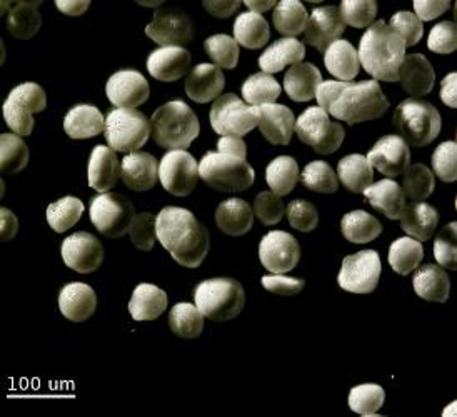
\includegraphics[height=5cm]{img/microscope_TiO2_particles.pdf}
\end{figure}

\paragraph{Spray-dry process}
Rutile (TiO$_{2}$) was ground to a powder of sub-microscopic particles. 
A suspension of these nanoparticles in ethanol was sprayed into flame. The average size of particles was determined by the solid concentration in the suspension, by feed rate and by gas flow.It immediately formed spherical droplets, which dried up and sintered in the hot air.  

The resulting particles were annealed in a furnace to further solidify. By the temperature of the furnace, the degree of recrystallization could be controlled: from microscopic grains (at around 1200  $^{\circ}$C) to a sphere consisting of few crystalline domains, which were apparent in electron microscope (annealed at\footnote{From personal communication with Dr. Patrick Mounaix} 1300--1400 $^{\circ}$C). Note the temperatures used are still far below the melting temperature of rutile (i.e. 1800 $^{\circ}$C).

Only the low-temperature annealed samples were measured by the terahertz spectroscopy in this thesis. The fine-grained rutile was assumed to be well approximated by an isotropic dielectric. The size of the constituent crystalline grains was estimated from the observation of one microsphere ground on a glass of a pollarisation microscope: unlike polycrystalline aggregates, single rutile monocrystals manifest as coloured particles due to their inherent birefringence. Therefore, the size of crystalline grains were determined in the order of few micrometers.

Similar TiO$_{2}$ microspheres are also available commercially (e.g. from Brace, GmbH), and to the author's knowledge, they are made with a similar process.

\paragraph{Microsphere pre-sieving and other treatment}
The annealed spheres required further processing, as described by {Dr.} U-Chan Chung: 
\textit{
(\ldots) As the spheres have been sintered at high
temperature, they have been separated from a platinum plate with a
small soft paintbrush followed by a light milling with a agathe
mortar. The goal was to separate the spheres that are welded to their
neighbours due to the sintering step. All the spheres were treated in
ultrasound-bath using ethanol as liquid phase. After natural drying,
the sieving was performed. (\ldots) square (or rectangular)
holes sieves were used. The meshes used were 106, 100, 53, 50, 40 and 38
micrometer. As a dry sieving step was performed, the particles were
light milled again in order to try to break possible agglomerates which
would not go through the mesh. This process was repeated 2-3 times and
a final wet sieving with ethanol was performed in order to "wash" the
spheres. No special measures were taken according to their shapes. (\ldots)
}


\paragraph{Theory of anisotropic sieves}
Triple sieving on commercial sieves in Bordeaux, weaved from stainless steel wire, did not provide narrow enough size distribution. We therefore developed detailed methods of sample refinement and characterisation. 

\begin{figure}[h] \caption{\textbf{a)} \textbf{b)} } \label{fg_sieve_pass_notpass} \centering 
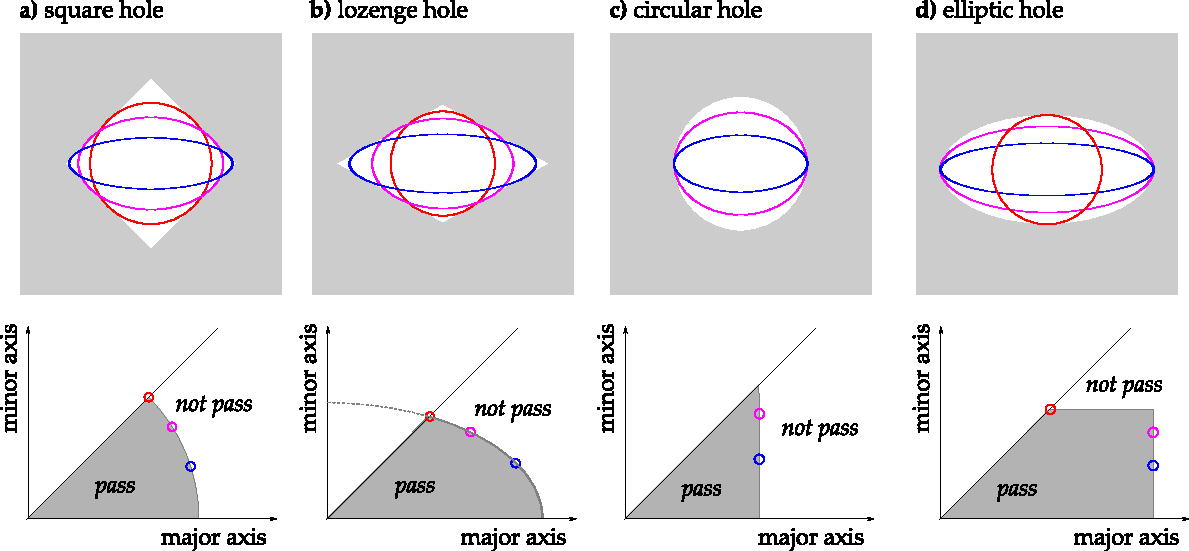
\includegraphics[width=\textwidth]{img/technology/sieve_pass_notpass.pdf}
\end{figure}
In the following, we approximated the dielectric particles by ellipsoids with three (generally different) half-axes $$r_a \leq r_b \leq r_c.$$ For the purpose of sieving, only the values of the shortest two axes, $r_a$ and $r_b$, decide whether the particle can pass through the sieve. The longest ellipsoid axis $r_c$ does not affect this, although it may influence the sieving speed. Therefore we can represent each 3-D particle with its projection on the smallest possible ellipse, which is described by its \textit{minor axis} $\equiv 2r_a$, and by its \textit{major axis} $\equiv 2r_b$. For a given shape of a hole in a homogeneous flat sieve, it is easy to determine which values of minor and major axes allow a particle to pass through, and which not. For a square sieve such area in the parameter space forms a disk around the center of origin (Fig. \ref{fg_sieve_pass_notpass}a). It can be shown that when the sieve is diagonally stretched, forming a lozenge hole shape, the area of spheres allowed to pass changes into an ellipse (Fig. \ref{fg_sieve_pass_notpass}b). When the hole shape is circular or elliptical, it is obvious that the area forms a part of a square or of a rectangle, respectively  (Fig. \ref{fg_sieve_pass_notpass}c,d).

The resonance frequency of a dielectric resonator depends on all three half-axes, $r_a \leq r_b \leq r_c$. In order to select as narrow size fraction as possible, one has to use double sieving: the above sieve not allowing the fraction of particles too big, the bottom sieve removing the fraction of particles too small. This is where the anisotropic hole shapes become useful -- the bottom sieve can exclude also all oblong particles with the difference of $r_a \leq r_b$ too big. This effect is illustrated in Fig. \ref{fg_double_sieving}, which also presents a comparison of using more usual sieves of square/lozenge holes with the effect of a couple of sieves of micromachined square/elliptic holes. Obviously, the latter approach better discriminates for the \textit{shape} of the ellipsoid. This advantage further gains on importance when the anisotropy of the sieve is low.
\begin{figure}[ht] \caption{\textbf{a)} \textbf{b)} } \label{fg_double_sieving} \centering 
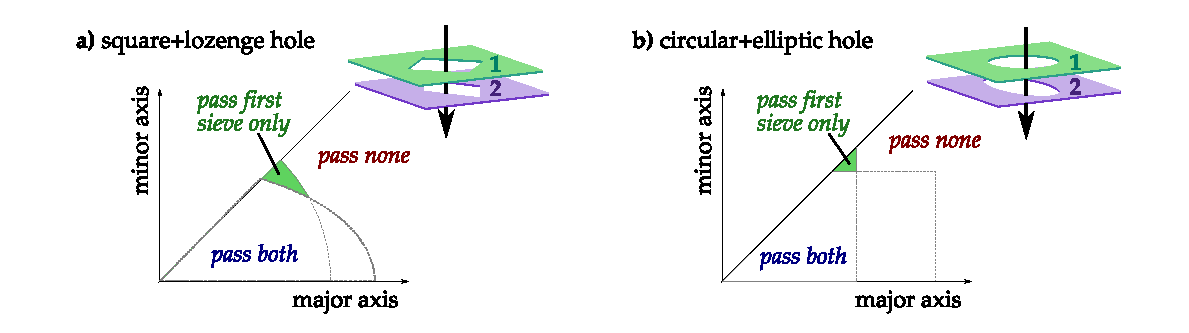
\includegraphics[width=\textwidth]{img/technology/sieve_double_sieving_fractions.pdf}
\end{figure}

% TODO 4x hole-sphere sketch  --->  maj-min binary funciton of (not)passing
It shall be noted that although we plotted a binary (\textit{pass}/\textit{not pass}) function in Figs. \ref{fg_sieve_pass_notpass} and \ref{fg_double_sieving}, the sieving speed greatly differs for different sizes of particles. This is due to lower probability of a particle passing, if its parameters are near the edge of possible-passing function. 
%For any finite sieving time, this obviously affects the statistics of particles passing the sieve, favoring the average size to be lower for short sieving times. The particles that are close to 
However, this particular fraction of particles is exactly what one is interested in during the high-accuracy sieving! The process must therefore run for long enough time, in the order of days, and with as high sieving speed as possible.

\paragraph{First sieving apparatus}
 %Finally, they were carefully sieved in many iterations, to select a size fraction as narrow as possible.
Employing the idea of anisotropic sieves from Fig. \ref{fg_double_sieving}a, we assembled the first prototype based on nylon sieves, as depicted in Fig. \ref{fg_sieving1}. Two glass containers were lathed of a 
% diam
glass tube, and on their bottom, nylon sieves were glued. The side of the sieve holes was 60$\pm$5 $\upmu$m, and while the above sieve was kept isotropic, the bottom one was stretched by ca. 20-25 \% in diagonal direction. The nylon mesh was woven, so the threads easily bent aside, allowing oversized particles either to pass or to get stuck permanently, blocking the sieve within few minutes. To resolve the latter problem, two additional narrow glass rings were cut, with much coarser sieves glued on the bottom, to allow little spherical springs bounce beneath the sieves and to loosen the particles that got stuck in the holes. A cover on top prevented the particles to jump out of the above container. Whole stack was carefully lowered into a test tube with a greater diameter, and vibrated by a tiny electric motor glued on the bottom.
\begin{figure} \caption{\textbf{a)}\textbf{b)}\textbf{c)} TODO input of unsorted microspheres}  \centering 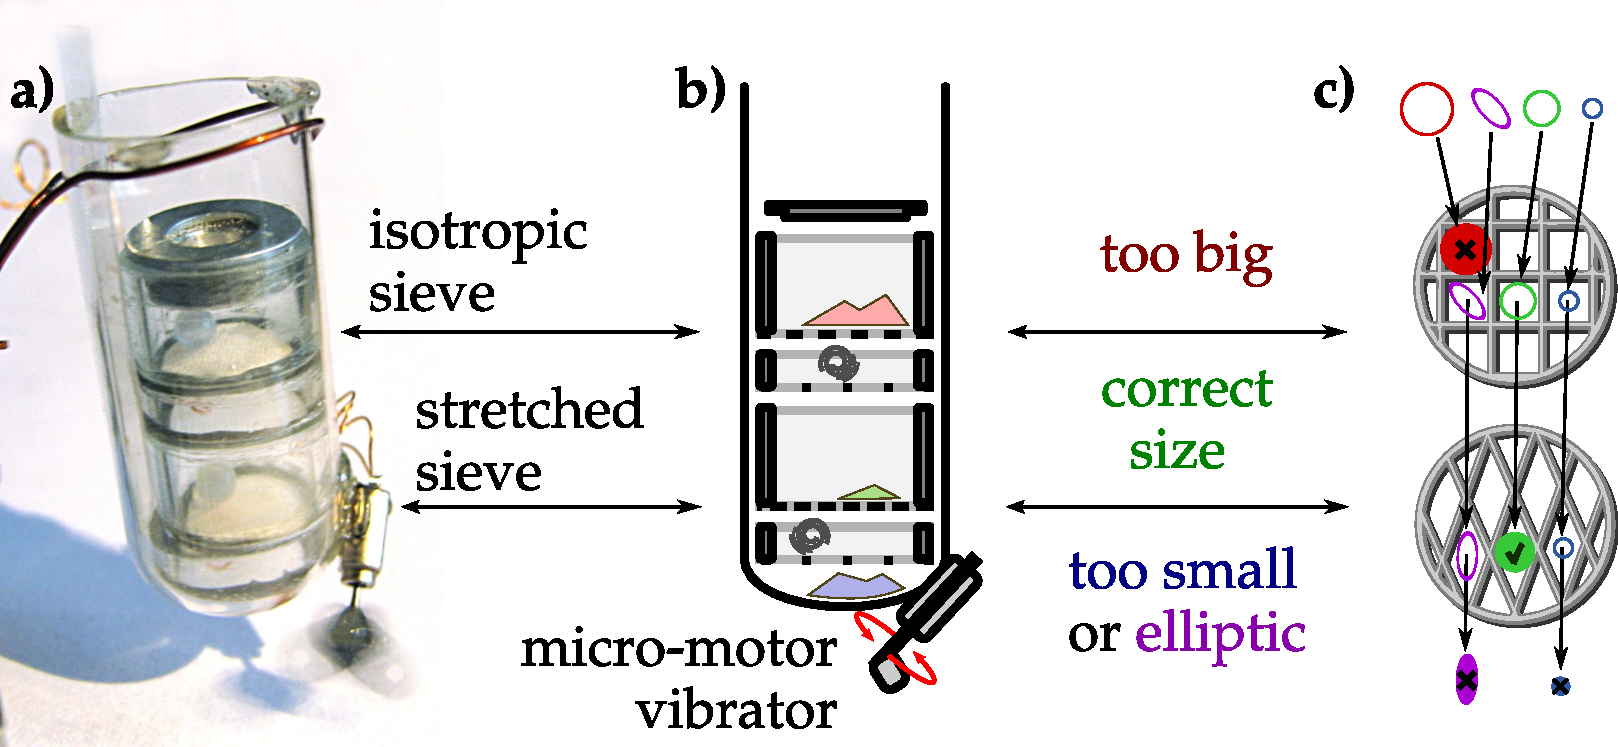
\includegraphics[width=12cm]{img/expe/sieving1.pdf} \label{fg_sieving1} \end{figure} 




\paragraph{Second sieving apparatus}
\begin{figure}[ht] \caption{\textbf{a)} A sketch of the acoustic sieving device, and \textbf{b)} a photograph thereof} \label{fg_sieving2} \centering 
\textbf{a)}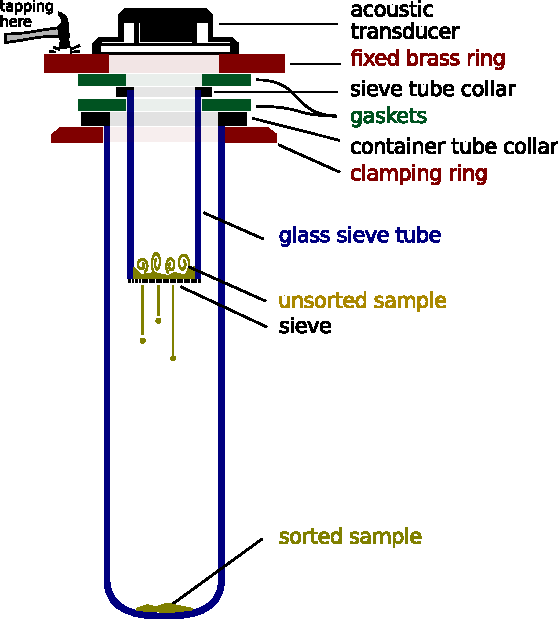
\includegraphics[height=8cm]{img/technology/sieve2_sieving_scheme.pdf}
\textbf{b)}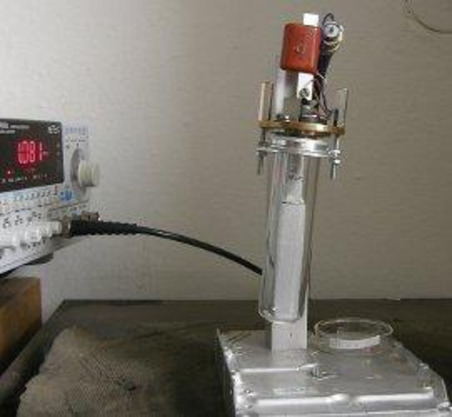
\includegraphics[height=8cm]{img/technology/sieving_m.pdf}
\end{figure}
The partially promising results and, more importantly, obvious deficiencies of the previous apparatus motivated building a second one depicted in Fig. \ref{fg_sieving2}.
Different from any other sieving apparatus known to the author, this one made use of intense vertical acoustic wave for the movement of particles. It consisted of two coaxial glass tubes: The inner tube, with outer diameter of 13 mm, had a round metallic sieve glued to its bottom, and on its upper end it was covered by a 20 mm acoustic transducer. The outer tube (90 mm long, outer diameter 26 mm) surrounded the inner one and had a round bottom, where the particles collected. 
The gaskets ensured that whole apparatus was tightly closed, preventing both sieved particles and sound from escaping. The brass ring with the transducer was fixed to a massive aluminum stand, and the rest of the structure was clamped to it by two M3 screws with nuts that allowed for easy disassembly. 

The key advantages of this novel approach are the following:
\begin{enumerate}
 \item{\textbf{The speed of sieving} is roughly proportional to the frequency at which the particles hit the sieve. The acoustic frequency of 1 kHz is rouhly two orders of magnitude higher than in usual commercialy available devices. The spheres are moreover continuously stirred, so it is ensured that a layer of over-sized particles does not occupy the sieve.} 
 \item{The upward air pressure \textbf{pulls out particles that got stuck in the sieve} in every period of acoustic vibration. This resolves the major issue of the previous prototype.} 
 \item{\textbf{Avoiding macroscopic vibrating parts}, except the membrane of a small acoustic transducer, allows the device to operate over multiple days without the risk of mechanical failure of any part.}
 \end{enumerate}


The outer tube acted as an acoustic resonator, greatly enhancing the effect of the sound when tuned to resonance around 750-900 Hz. These frequencies obviously correspond to the fundamental acoustic resonance, as the quarter-wavelength is the range from 91 to 110 mm. 

%TODO The power of the sinewave feeding the device was limited by the parameters of the acoustic transducer
A practical deficiency of this setup was that the upper opening of the transducer radiated relatively intense sound during operation. We resolved this potential issue by covering whole apparatus by a robust glass bell jar.

With the acoustic power and frequency correctly adjusted, the particles formed a cloud 5--10 mm high. One difficulty arose from that the small particles tend to attach to the surface of glass or metal, probably due to electrostatic charges on their surface. While at an average particle radius $\rho = 50$ $\upmu$m this effect was rather marginal and transient, it took only few seconds of sieving for $\rho = 20$ $\upmu$m particles to immobilize permanently on any surface. It has however proven efficient to tap the upper brass ring, as the vibration released most spheres, effectively renewing the sieving process. To ensure unattended sieving for a timespan in order of days, we added a little motorized hammer with a timing circuit. % todo add photo of the hammer

The amount of particles in one batch was limited to ca. 10--20 mm$^{3}$, otherwise the sieve would be covered with a layer too thick, which could not be efficiently lifted by the acoustic pressure.
It could however be remedied by tilting the apparatus. With a tilt of 5--10 degrees, the bulk of particles then accumulated near one side, leaving most of the sieve surface free for sieving the moving fraction of particles. According to the small amount of particles required for the terahertz spectroscopy measurements, it is however advisable to sort a batch in order of 1--3 mm$^{3}$.

\subsection{Automatic determination of microparticle statistics}
\begin{figure}[ht] \caption{\textbf{a)} A section of a microphotograph of sample before sieving, \textbf{b)} the corresponding identification of particles in ImageJ} \label{fg_microphoto} \centering 
\textbf{a)}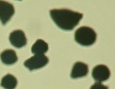
\includegraphics[height=5cm]{img/technology/imagej_photo.pdf}
\textbf{b)}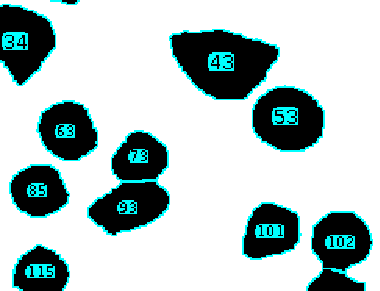
\includegraphics[height=5cm]{img/technology/imagej_found.pdf}
\end{figure}

We developed a numerical method to measure the histogram of size distribution of the particles based on a calibrated microphotograph of the sample such as in Fig. \ref{fg_microphoto}1. This enabled to assess the sieving precision and also to predict the realistic signal by simulation.
\add{ TODO}
% TODO  add the 4-fold png figure from web

\subsection{Laser micro-machining of sieves and fish-net metamaterial layers}
\begin{figure}[ht] \caption{\textbf{a)} Laser micromachining the steel sieve, and \textbf{b)} the resulting sieves} \label{fg_microfab} \centering 
\textbf{a)}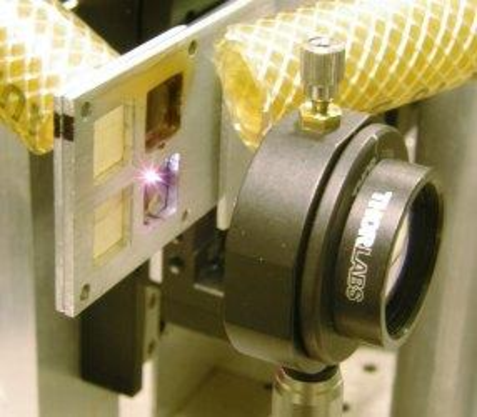
\includegraphics[height=5cm]{img/technology/sieve2_drilling_m.pdf}
\textbf{b)}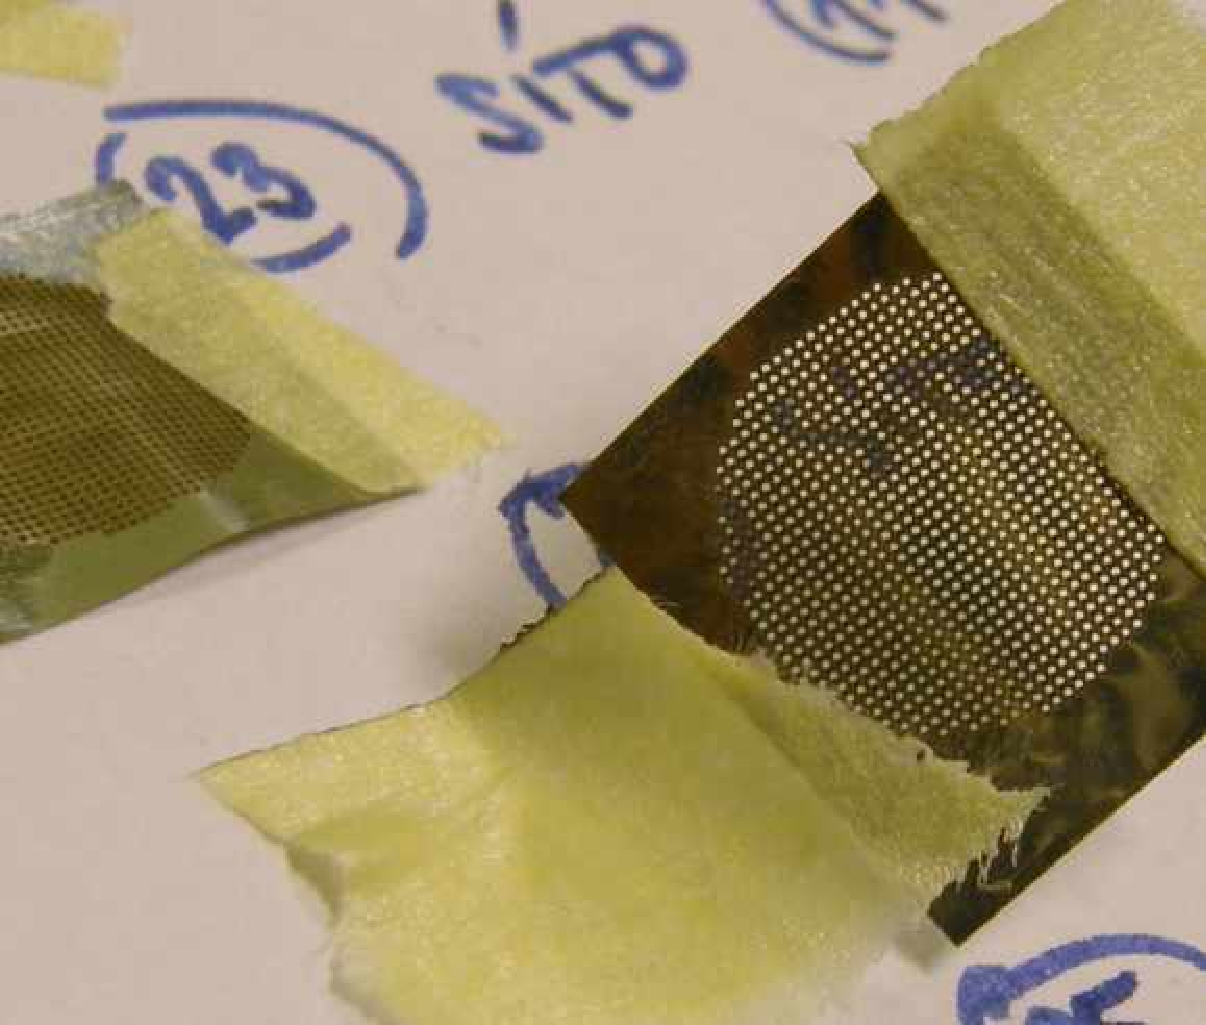
\includegraphics[height=5cm]{img/technology/steel_sieve_on_paper.pdf}
\end{figure}

To achieve the required precision of sieving, we fabricated the sieves by femtosecond laser drilling of 20 $\upmu$m thick stainless steel sheets (Fig. \ref{fg_microfab}). 
%These sieves then were employed in a device that subjected the microsphere sample to acoustic vibrations, improving the speed of the demanding sieving process to acceptable level (Fig. \ref{fg_microfab}b,c).
\add{ TODO}


\add{Owing to the homogeneous broadening of the resonator resonance, caused by intrinsic losses of TiO$_{2}$, further sieving appears to lack any purpose. Not only this project broadens the numerous group of technically successful research projects pointed in utterly wrong direction, it also classifies into the lamentable subgroup of effort that could be entirely avoided if open and honest scientific discussion took place about the inherent problems. In this case, particularly, in all related papers it should be openly stated, that the dielectric losses of TiO2 prevent building any applicable volume metamaterial, no matter how accurately the resonators are prepared.}






%A rough list of the most important phenomena follows. 
%\begin{table}[ht]   \caption{}  \label{tb_} \centering 
%\begin{tabular}{lcr}
 %\toprule
%Frequency $\omega_0/(2\pi)$         & Contribution $\Delta\varepsilon_r$ & Physical phenomenon	\\
 %\hline
%---									& 0--10000 &	& Rotation of polar molecules	\\
%1 THz -- 30 THz						& & Vibration of atomic lattice	\\
%200 THz - 1000 THz					& &	\\
 %\bottomrule
 %\end{tabular} \end{table}
%\begin{enumerate}
 %\item{In the low frequency and microwave range (up to 1 THz), rotation and reorganisation of polar molecules plays the major role in the medium polarizability. } 
 %\item{Depending on the hardness and density of the medium, the lattice vibrates at frequencies between 1 and 30 THz.} 
 %\item{The frequencies corresponding to  electron motions of solids are in near-infrared, optical or ultraviolet ranges (roughly 200-1000 THz).}
 %\end{enumerate}
%If the medium is conductive, 
